\documentclass[lettersize,journal]{IEEEtran}
\usepackage{amsmath,amsfonts}
\usepackage{algorithmic}
\usepackage{algorithm}
\usepackage{array}
% \usepackage[caption=false,font=normalsize,labelfont=sf,textfont=sf]{subfig}
\usepackage{caption}
\usepackage{subcaption}
\usepackage{textcomp}
\usepackage{stfloats}
\usepackage{url}
\usepackage{booktabs}
\usepackage{verbatim}
\usepackage{graphicx}
\usepackage{xcolor}
\graphicspath{{../gfx/}}
\usepackage{cite}
% \hyphenation{op-tical net-works semi-conduc-tor IEEE-Xplore}

% \usepackage{draftwatermark}
% \SetWatermarkScale{.85}
% \SetWatermarkText{DRAFT}

\newcommand{\rc}[1]{\textcolor{red}{#1}}
\newcommand{\dg}[1]{\textcolor{purple}{#1}}
\newcommand{\ak}[1]{\textcolor{teal}{#1}}

% \renewcommand{\floatpagefraction}{1}
% \renewcommand{\topfraction}{1}
% \renewcommand{\bottomfraction}{1}
% \renewcommand{\dbltopfraction}{1}
% \renewcommand{\textfraction}{0} % allow minimal text w. figs
% %   Parameters for FLOAT pages (not text pages):
% \renewcommand{\floatpagefraction}{0.999}    % require fuller float pages % N.B.: floatpagefraction MUST be less than topfraction !!
% \renewcommand{\dblfloatpagefraction}{0.999} % require fuller float pages

\begin{document}

\title{Co-design of a wave energy converter through bi-conjugate impedance matching }
{}
\author{Sandia National Labs (some order of Alicia, Daniel, Dom, Giorgio, Ryan)
        % <-this % stops a space
% \thanks{This paper was produced by the IEEE Publication Technology Group. They are in Piscataway, NJ.}% <-this % stops a space
\thanks{Manuscript received XX; revised XX}}

% The paper headers
\markboth{IEEE Transactions on Sustainable Energy}%
{Author1 \MakeLowercase{\textit{et al.}}: Title}

% \IEEEpubid{0000--0000/00\$00.00~\copyright~2021 IEEE}
% Remember, if you use this you must call \IEEEpubidadjcol in the second
% column for its text to clear the IEEEpubid mark.

\maketitle

\begin{abstract}
As with other oscillatory power conversion systems, wave energy converter design can be understood as an impedance matching problem.
By representing the wave energy converter as a multi-port network, two separate, but related, impedance matching conditions can be established.
Satisfying these conditions maximizes power transfer to the load.
In practice, we may use these impedance matching conditions to influence system (hull, power take-off, controller, mooring, etc.) design.
To this end, this paper considers some example wave energy converter design applications with the help of the impedance matching conditions.
\end{abstract}

\begin{IEEEkeywords}
wave energy converter (WEC), control co-design, impedance matching
\end{IEEEkeywords}

% ------------------------------------------------------------------
\section{Introduction}

% \rc{
% \begin{itemize}
%         \item XX-Simplification for non-oscillatory inputs (e.g., wind turbine)
%         \item XX-Adding inertia vs. spring
%         \item XX-Why do we show $I_{\textrm{out}}$ into the PTO by convention? \url{https://en.wikipedia.org/wiki/Two-port_network#ABCD-parameters}
%         \item XX-Shouldn't we have $Z_{12} = Z_{21}$ if the PTO is passive (see, e.g., \url{https://ocw.mit.edu/courses/6-061-introduction-to-electric-power-systems-spring-2011/d79822ef5fbdb21b1c44e1b3b8282453_MIT6_061S11_ch1.pdf})?
%         \item XX-losses vs. reflections
%         \item XX Th\'{e}venin vs. two-port
%         \item XX one- vs. two-port
%         \item Kirchhoff's laws
%         \item XX Kirtley: ``If the networks are linear and passive (i.e. there are no dependent sources inside), they also exhibit the property of reciprocity. In a reciprocal network, the transfer impedance or transfer admittance is the same in both directions''
%         \item A two-port network has four variables with two of them being independent. If one of the ports is terminated by a load with no independent sources, then the load enforces a relationship between the voltage and current of that port. A degree of freedom is lost. The circuit now has only one independent parameter. The two-port becomes a one-port impedance to the remaining independent variable. (\url{https://en.wikipedia.org/wiki/Two-port_network#Collapsing_a_two-port_to_a_one_port})
%         \item Maximum power transfer theorem (\url{https://en.wikipedia.org/wiki/Maximum_power_transfer_theorem})
%         \item \url{https://stuff.mit.edu/afs/athena/course/2/2.151/www/index.html}
%         \begin{itemize}
%                 \item ``The process of energy conversion between domains is known as transduction and elements that convert the energy are defined to be transducers''
%                 \item The two-port transducer is a lossless element; for many physical systems it is necessary to formulate a model for a transducer that consists of an ideal two-port coupled with one or more one-port elements to account for any energy storage and dissipation that occurs in the real transducer.
%         \end{itemize}
%         \item through and across variables (wikipedia)
%         \begin{itemize}
%                 \item across: A variable whose value is determined by measuring a difference of the values at two extreme points of an element; thus voltage is a difference in two levels of potential.
%                 \item through: A variable transmitted through an element. For example, the torque applied at one side of a stem is transmitted through this one to the other side.
%         \end{itemize}
%         \begin{itemize}
%                 \item Maximum power transfer to load (not maximum efficiency)
%         \end{itemize}
% \end{itemize}}


Wave energy converters (WECs) must be designed to capture a purely oscillatory power input.
Amongst other energy generation technologies (e.g., wind turbines, hydro-electric dams, nuclear power plants), this is a unique characteristic.
However, given the broad application of AC electrical power, there are useful tools at the disposal of a WEC designer for maximizing useful power output.

The concept of impedance matching to minimize reflections has been applied in wave energy since at least the 1970s \cite{Falnes:1980aa}.
For reasons that are unclear, the concept was mostly only applied to the conversion stage for transferring power from the waves to the WEC's hull/input of the power take-off (PTO) system.
As will be discussed in further detail in this paper, disregarding the subsequent power conversion stages between mechanical power on the hull and useful (e.g., electrical) power at the output of the machine has a number of adverse repercussions.

This concept of transferring power between different stages is illustrated in \figurename~\ref{fig:wec_as_multiport_power_transfer_stages}.
The ultimate goal of a WEC is to deliver power to a load.
In a WEC designed to produce electrical power, this would represent the electrical outputs from a motor/generator.
Because the source power is purely oscillatory, the power flow between the stages in \figurename~\ref{fig:wec_as_multiport_power_transfer_stages} is shown to be bi-directional in general.
In fact, the optimal condition requires that half the power be reflected \rc{XX-cite}.
The conditions that ensure this optimal power transmission by minimizing reflections are shown at the top of \figurename~\ref{fig:wec_as_multiport_power_transfer_stages}.
The first impedance matching condition in \figurename~\ref{fig:wec_as_multiport_power_transfer_stages} ($Z_{\textrm{in}} = Z_i^*$) is generally well-known and widely applied, although using somewhat different notation as the input/output distinction within the PTO is not widely utilized.
The second impedance matching condition in \figurename~\ref{fig:wec_as_multiport_power_transfer_stages} ($Z_{\textrm{out}} = Z_\ell^*$) is mostly ignored and/or lumped with first condition, thus limiting performance.

\begin{figure}[tb]
        \centering
        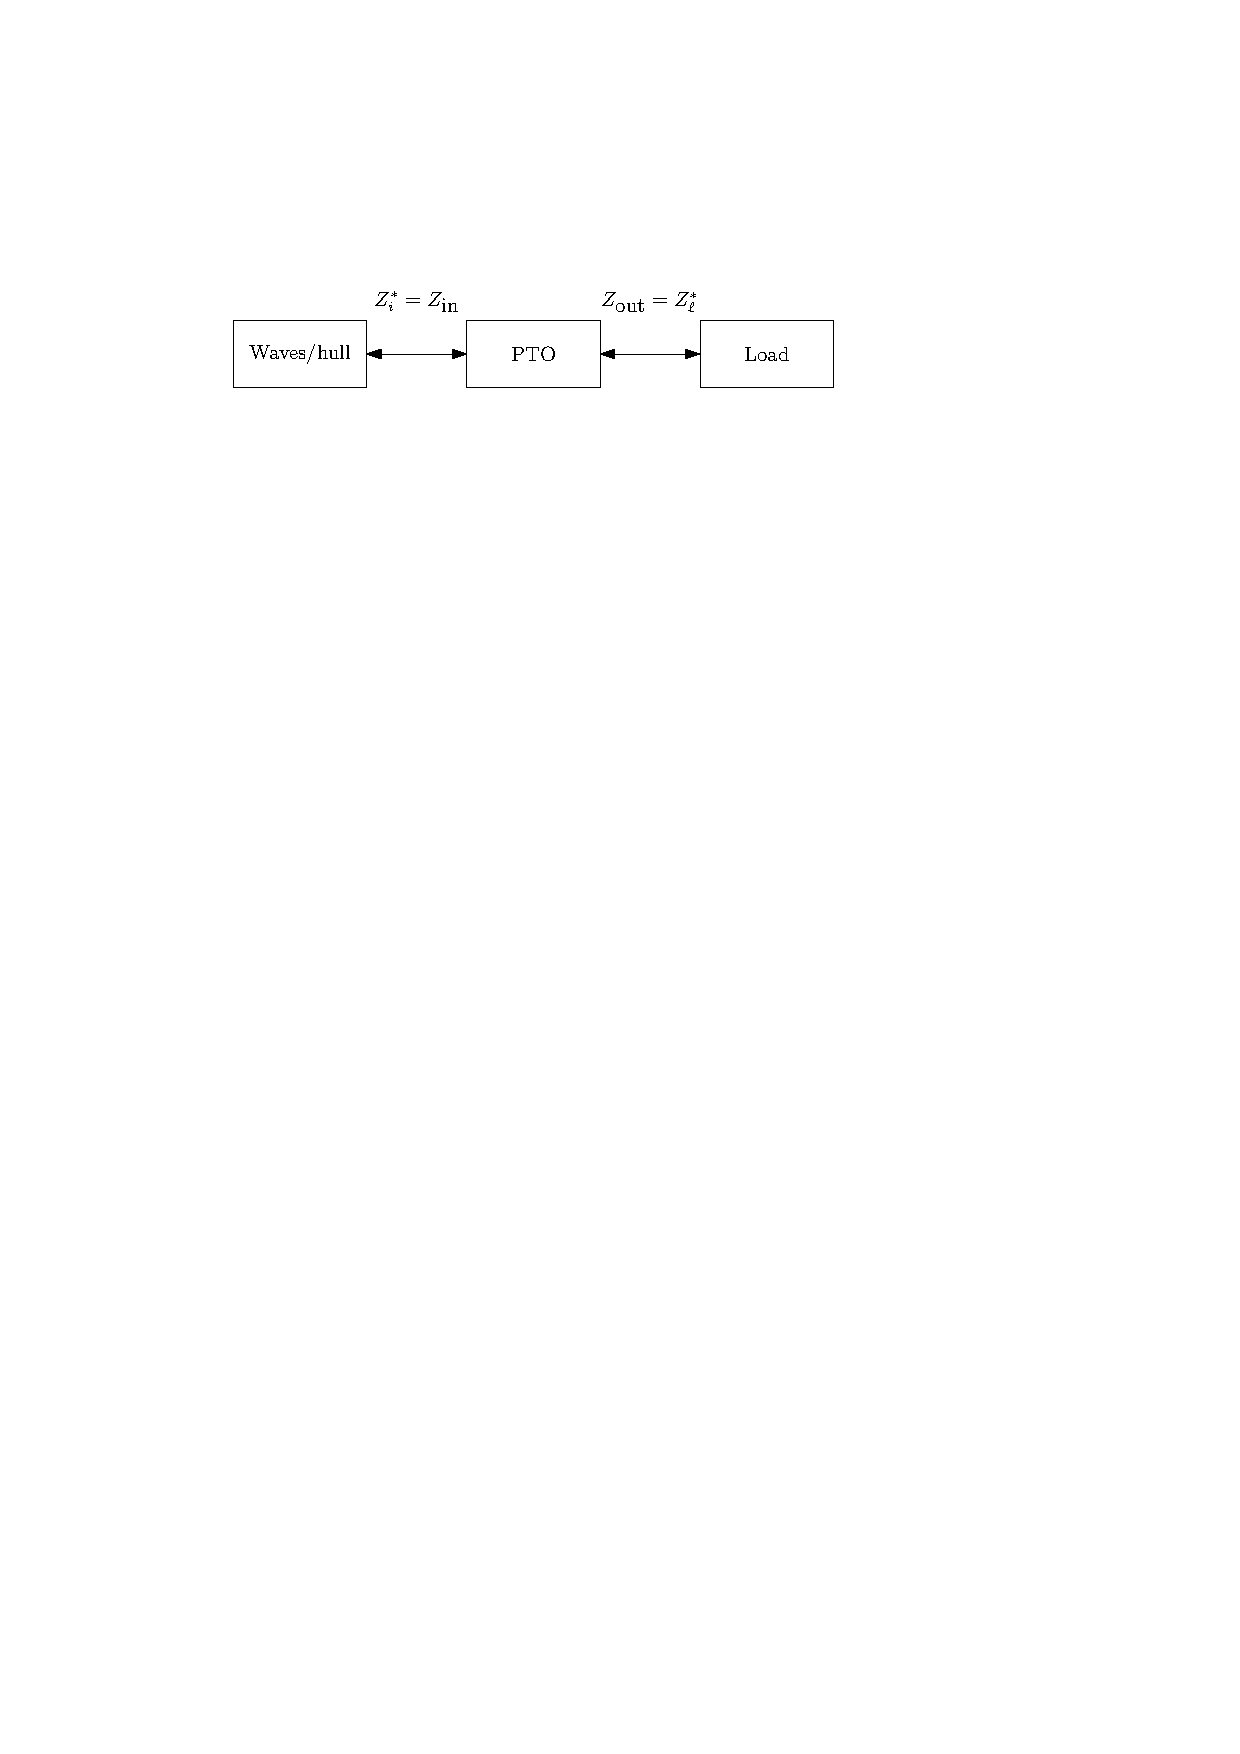
\includegraphics[width=1\columnwidth]{wec_as_multiport_power_transfer_stages.pdf}
        \caption{XX}
        \label{fig:wec_as_multiport_power_transfer_stages}
\end{figure}

Power delivered to the load is affected by both losses and reflections in this system.
These two effects are distinct and must addressed with an appreciation as such.
Losses are due to friction or electrical resistance -- this effect is often more intuitive and will not be discussed here in detail.
Reflections are due to a mismatch in the system impedances.
%%% Dom feels this is a bit of an over-simplification maybe better suited for a discussion section later on. While minimizing losses is important, friction and resistance are contributors to the real part of impedance and, especially in absence of other contributors (gear ratio, Kt) being called out explicitly I think this might yield confusion.
This paper will further explore concepts of bi-conjugate impedance matching in wave energy previously raised by \cite{Bacelli:2021aa}, with the goal of generating a more practical understanding for the utility and application of this theory.
First, an basic review of network modeling and elements is presented (Section~\ref{sec:two_port_networks}).
Next, this framework is applied to a WEC and used to formulate the bi-conjugate impedance matching condition (Section~\ref{sec:modeling_a_direct_drive_wec}).
This framework is then applied in a number of illustrative case-studies (Section~\ref{sec:illustrative_examples}).

% % ------------------------------------------------------------------
% \section{Bi-conjugate impedance matching}\label{sec:bi_conjugate_impedance_matching}
% We may express the dynamics of a WEC using an intrinsic impedance ($Z_i$) that relates the velocity ($v$) to the external forces: an ``excitation'' force from incoming waves ($F_{\textrm{exc}}$) and a force from the PTO ($F_{\textrm{pto}}$) \cite{Falnes:2002aa}.

% \begin{equation}
%         Z_i v = F_{\textrm{exc}} - F_{\textrm{pto}}
%         \label{eq:intrinsic_impedance_eom}
% \end{equation}

% \noindent{}The intrinsic impedance can be defined by elements of the linear potential flow free surface hydrodynamics (see, e.g., \cite{Newman:1978aa}).

% \begin{equation}
%         Z_i(\omega) = B(\omega) + b_f + j \left( \omega{}(m + A(\omega)) - \frac{K_{h}}{\omega}\right)
% \end{equation}

% \noindent{}Here, $A(\omega)$ is the added mass, $B(\omega)$ is the radiation damping, $K_h$ is the hydrostatic stiffness, $b_f$ accounts for linear friction effects, and $m$ is the rigid body inertia.
% The imaginary unit is $j$ and $\omega$ is the angular frequency.

% Much has been written about \eqref{eq:intrinsic_impedance_eom} and how to design a controller for $F_{\textrm{pto}}$ such that \emph{mechanical power} is maximized (see, e.g., \cite{Coe2020a} \rc{XX-cite others}).
% Within this approach to maximize mechanical power, there is an implicit assumption that the dynamics of the PTO can be decoupled from the hydrodynamic problem and, consequently, such a design will also maximize \emph{useful power} at the load (refer back to \figurename~\ref{fig:wec_as_multiport_power_transfer_stages}).

% ------------------------------------------------------------------
\section{Two-port networks}\label{sec:two_port_networks}
To consider the complete problem, without the faulty assumption that PTO dynamics may be decoupled from the hydrodynamic system, it is expedient to utilize the two-port network model popular in electronics and microwave systems \cite{Marrocco:2008aa}.
We may describe the system with a two-port impedance model, relating the effort ($e_i$) and flow ($q_i$) at each port (see \figurename~\ref{fig:wec_as_multiport_general_two_port_network}).
The products of the effort and flow variables on each port is power.
Note also the sign conventions illustrated in \figurename~\ref{fig:wec_as_multiport_general_two_port_network}, which result in a convention of power flow into the two-port network from both sides equal zero and the two-port network is lossless. 

\begin{figure}[tb]
        \centering
        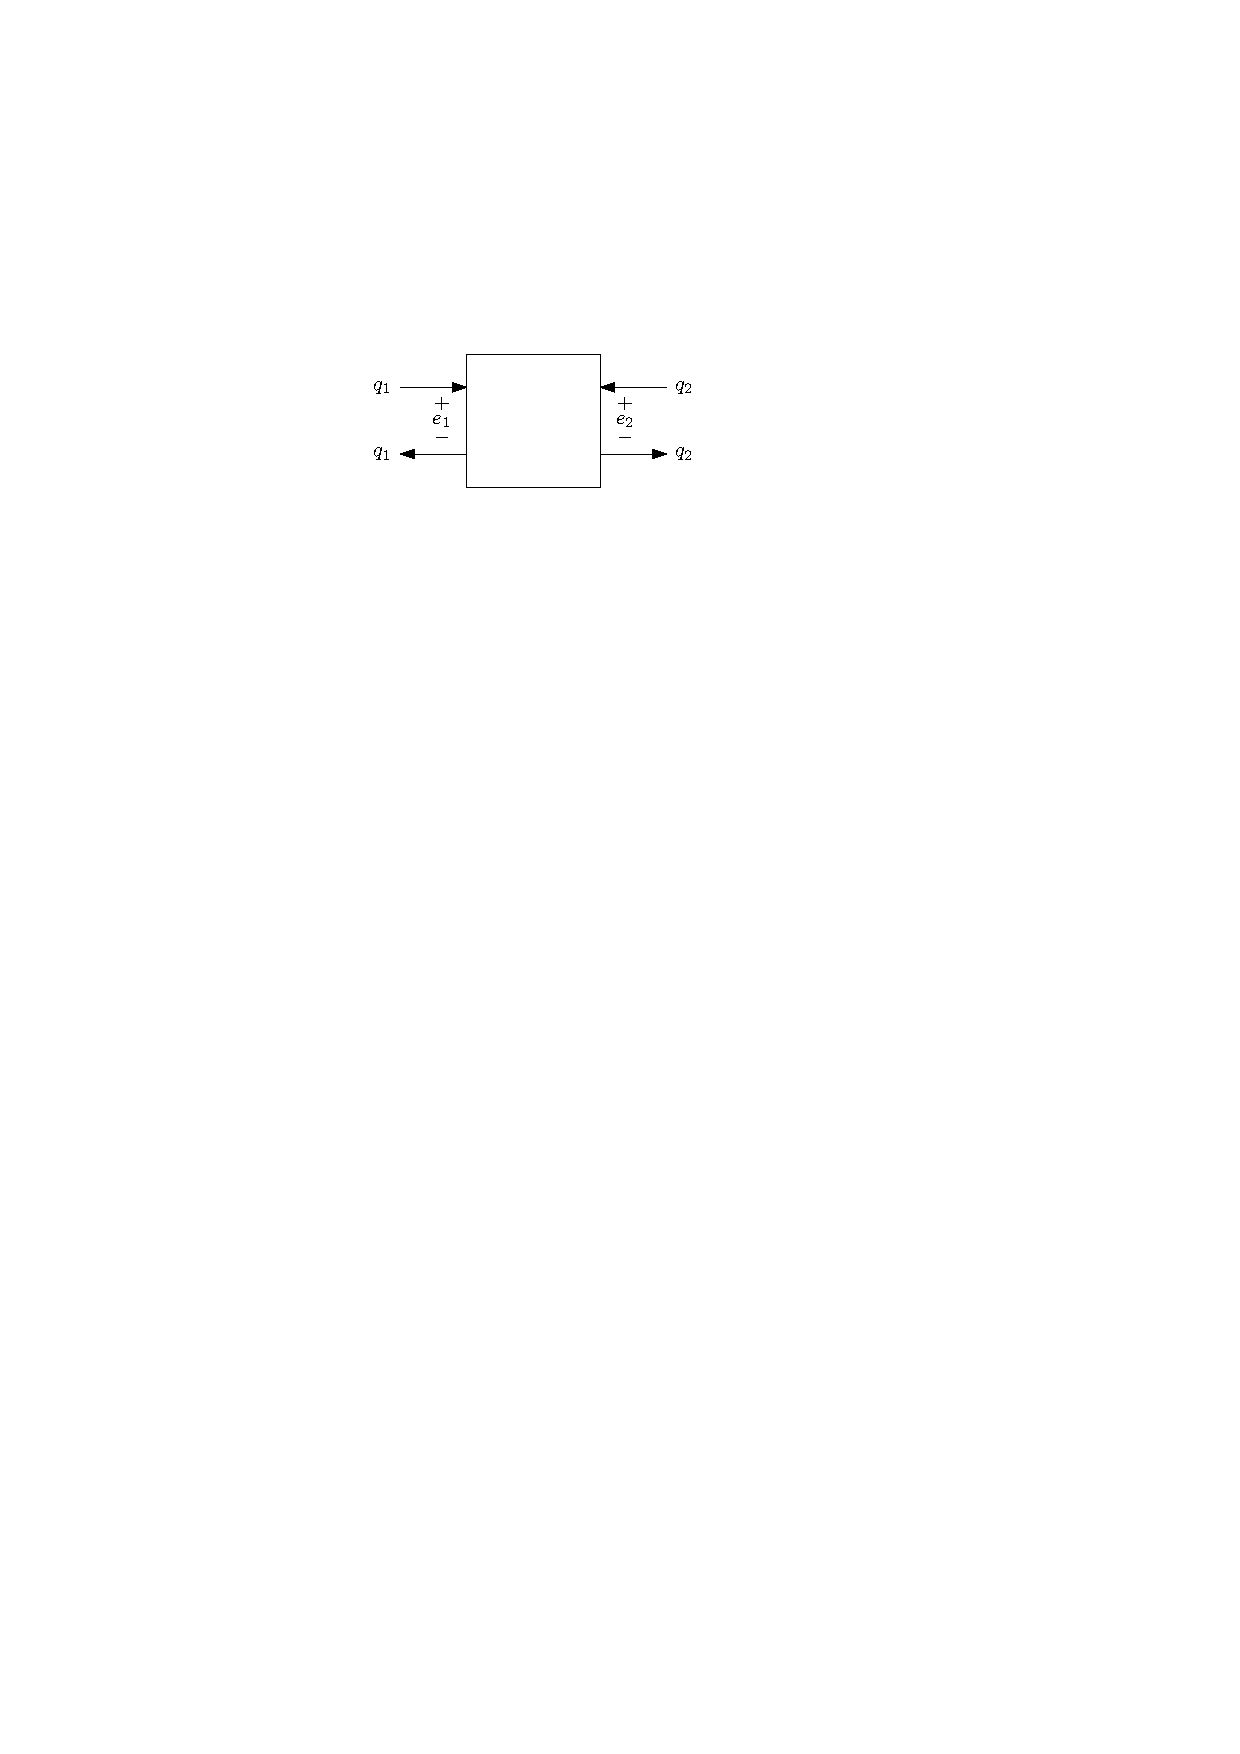
\includegraphics[width=0.75\columnwidth]{wec_as_multiport_general_two_port_network.pdf}
        \caption{General two-port network definition showing effort ($e_i$) and flow ($q_i$) at each port.}
        \label{fig:wec_as_multiport_general_two_port_network}
\end{figure}

\begin{equation} \label{eq:Z_mat_def_general}
        \begin{bmatrix} e_1 \\ e_2 \end{bmatrix} = \begin{bmatrix} Z_{11} & Z_{12} \\ Z_{21} & Z_{22} \end{bmatrix} \begin{bmatrix} q_1 \\ q_2 \end{bmatrix},
\end{equation}

\noindent{}The elements of any two-port impedance matrix may be defined as follows \cite{Frickey:1994aa}.

\begin{subequations} \label{eq:Z_mat_elements_def}
        \begin{align}
                Z_{11}& = \frac{e_1}{q_1} \bigg \vert_{q_2=0} \label{eq:Z_mat_elements_def_Z11} \\[1em]
                Z_{12}& = \frac{e_1}{q_2} \bigg \vert_{q_1=0} \label{eq:Z_mat_elements_def_Z12} \\[1em]
                Z_{21}& = \frac{e_2}{q_1} \bigg \vert_{q_2=0} \label{eq:Z_mat_elements_def_Z21} \\[1em]
                Z_{22}& = \frac{e_2}{q_2} \bigg \vert_{q_1=0} \label{eq:Z_mat_elements_def_Z22}
        \end{align}
\end{subequations}

In addition to the ``impedance form'' shown in \eqref{eq:Z_mat_def_general}, there are many equivalent formulations for modeling two-port networks \cite{Frickey:1994aa}.
Specific formulations can be easier to work with depending on the task at hand.
In this paper, we will also utilize the ``$ABCD$ form'' (also sometimes referred to as chain, cascade, or transmission form):

\begin{equation}
        \label{eq:abcd_mat_def_general}
        \begin{bmatrix} e_1 \\ q_1 \end{bmatrix}
        = 
        \begin{bmatrix} A & B \\ C & D \end{bmatrix}
        \begin{bmatrix} e_2 \\ - q_2 \end{bmatrix}
\end{equation}

\noindent{}Similarly to \eqref{eq:Z_mat_elements_def}, the elements of the $ABCD$ matrix are defined as follows.

\begin{subequations} \label{eq:abcd_mat_elements_def}
        \begin{align}
                A = \frac{e_1}{e_2} \bigg \vert_{q_2=0} \label{eq:abcd_mat_elements_def_a} \\[1em]
                B = - \frac{e_1}{q_2} \bigg \vert_{e_2=0} \label{eq:abcd_mat_elements_def_b} \\[1em]
                C = \frac{q_1}{e_2} \bigg \vert_{q_2=0} \label{eq:abcd_mat_elements_def_c} \\[1em]
                D = - \frac{q_1}{q_2} \bigg \vert_{e_2=0} \label{eq:abcd_mat_elements_def_d}
        \end{align}
\end{subequations}

\noindent{}Note that the impedance form and $ABCD$ form matrix elements are explicitly interrelated (see, e.g., \cite{Frickey:1994aa}).
For example, we may relate the impedance matrix and $ABCD$ as

\begin{equation}
        \begin{bmatrix}
                Z_{11} & Z_{12} \\ Z_{21} & Z_{22}
        \end{bmatrix}
        =
        \frac{1}{C}
        \begin{bmatrix}
                A & \Delta\left[ ABCD \right] \\ 1 & D
        \end{bmatrix} ,
\label{eq:abcd_to_Z}
\end{equation}

\noindent{}where $\Delta\left[ ABCD \right]$ is the determinant of the $ABCD$ matrix.
From \eqref{eq:abcd_to_Z}, we can see that some representations may be undefined for certain two-port elements (e.g., if $C=0$ in the $ABCD$ form, the impedance form will be undefined).

An important property of a two-port element is that it can be collapsed to a one-port element if one of the ports is terminated with a load and has no independent sources.
Whereas the general two-port element has four variables, two of which are independent, in the scenario where one port of terminated with a load, the system losses a degree of freedom.
Thus, in this case, we may simplify the system as a one-port element (i.e., a single impedance).

Transformers and gyrators (see \figurename~\ref{fig:wec_as_multiport_transformer_gyrator}) are two fundamental classes of two-port networks worthy of further discussion.

\begin{figure}[tb]
        \centering
        % 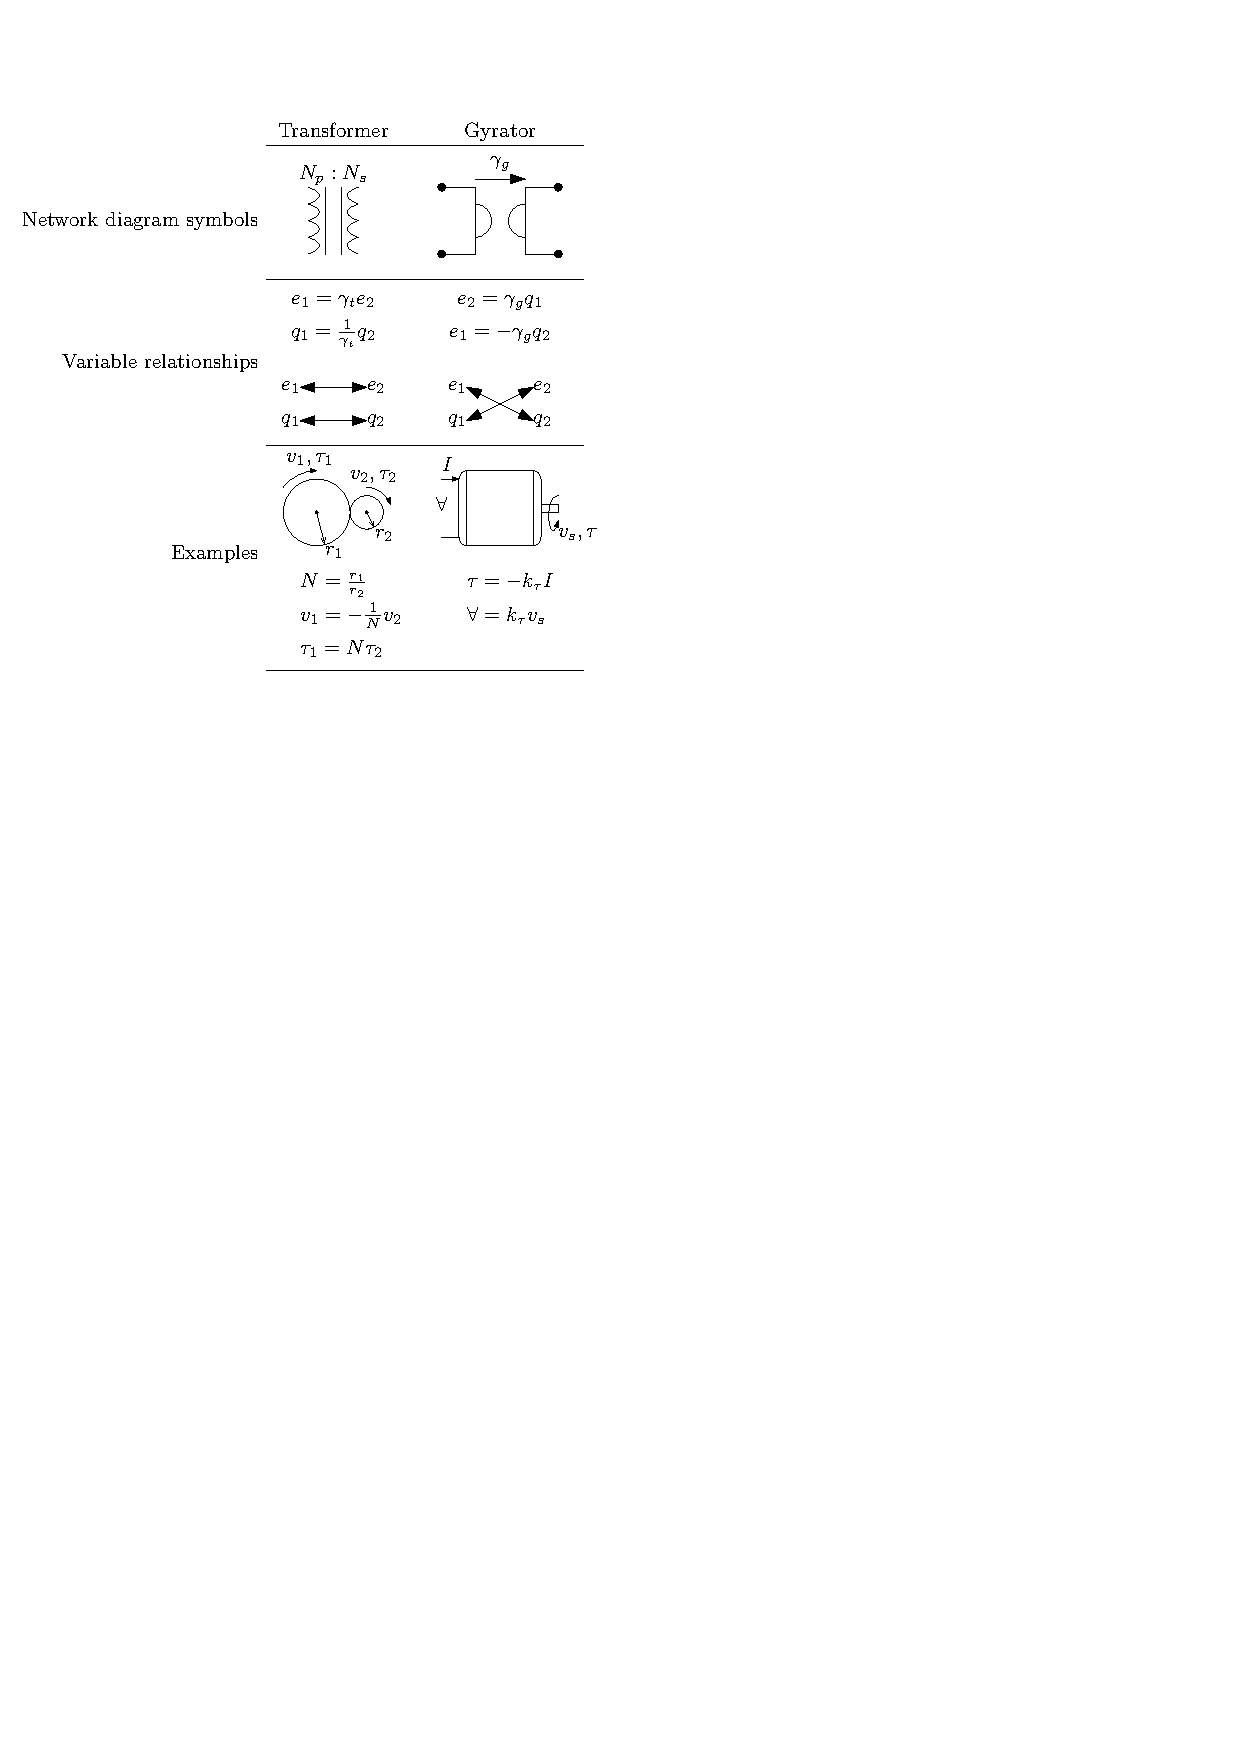
\includegraphics[width=\columnwidth]{wec_as_multiport_transformer_gyrator.pdf}   
        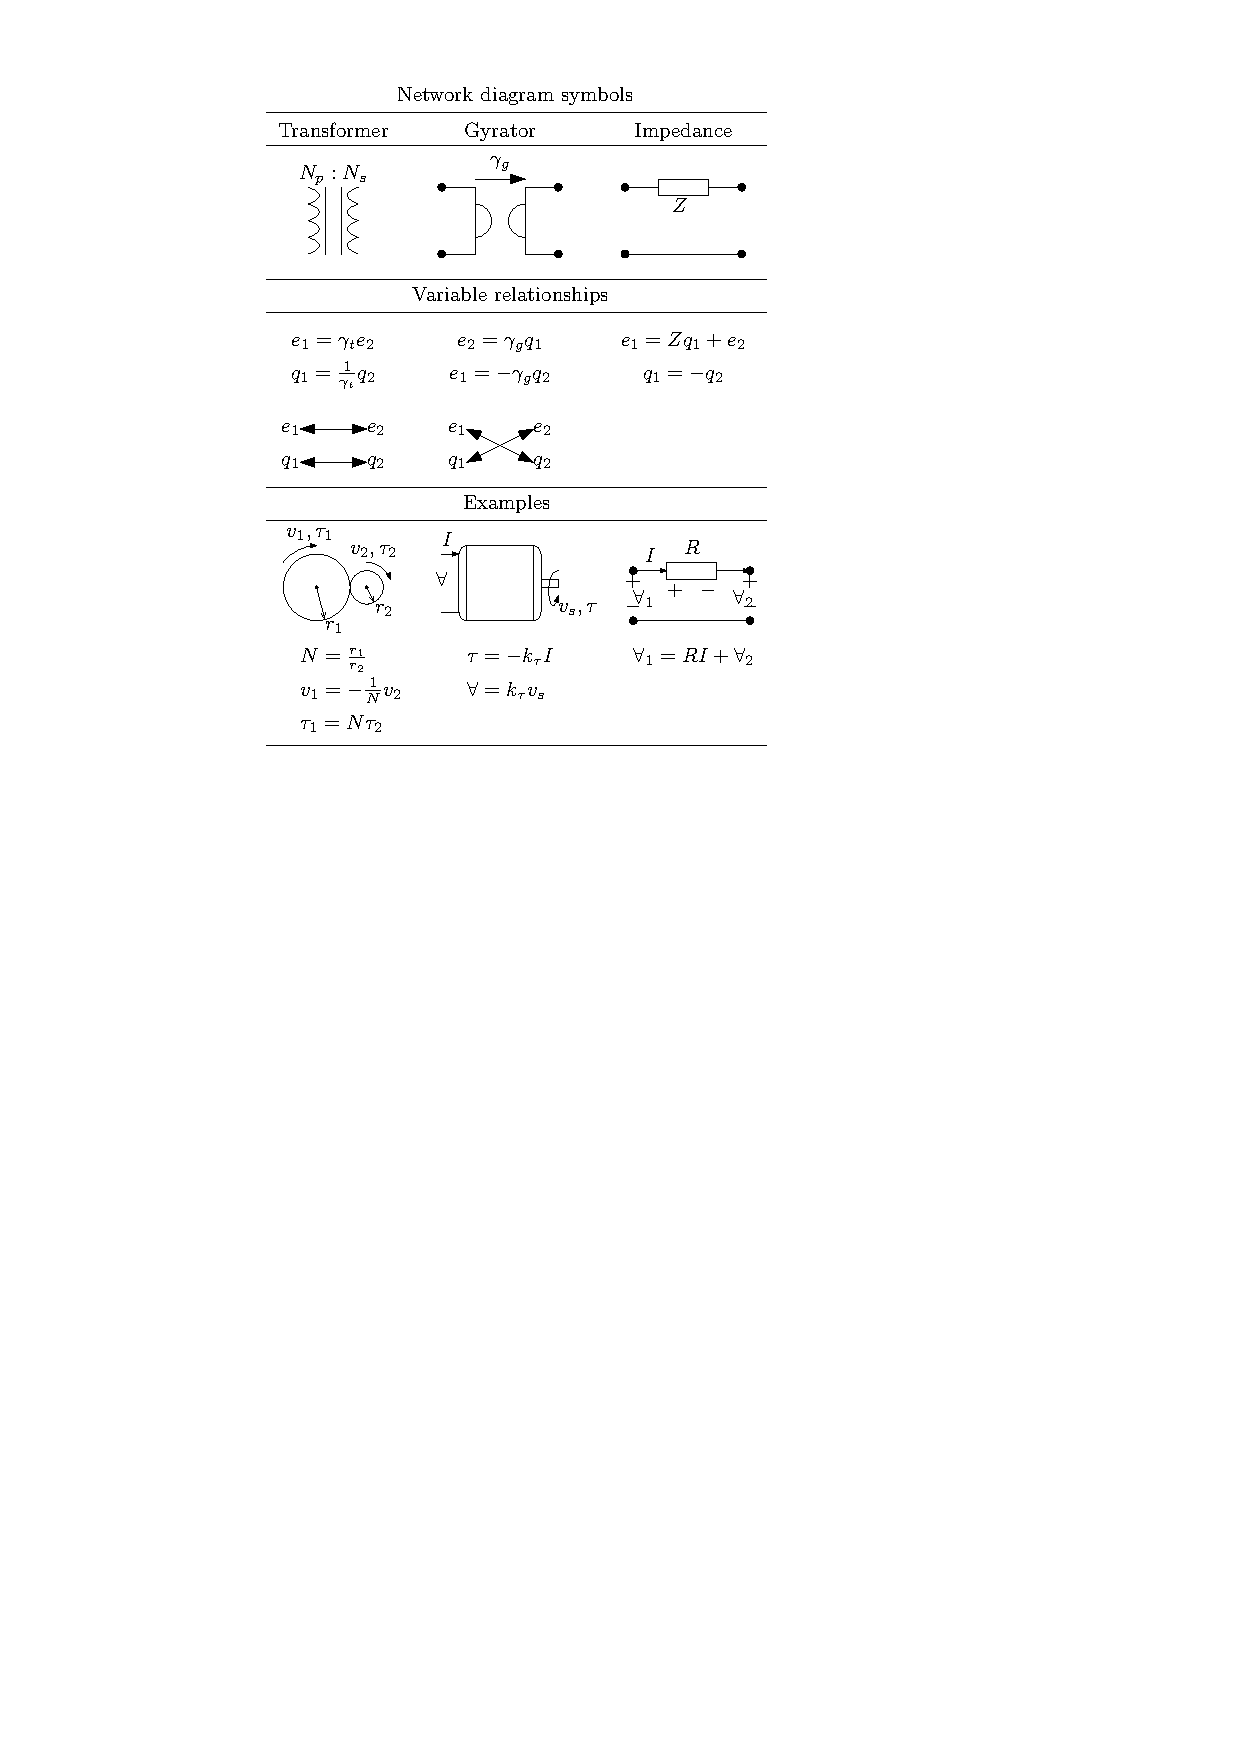
\includegraphics[width=\columnwidth]{wec_as_multiport_transformer_gyrator_impedance.pdf}
        \caption{Transformer and gyrator diagrams and mathematics.}
        \label{fig:wec_as_multiport_transformer_gyrator}
\end{figure}

% ------------------------------------------------------------------
\subsection{Transformers}\label{sec:trasnformers}
Electric transformers are widely known and understood to convert between different voltage levels.
For an ideal transformer, we may define a constant $\gamma_{t}$ that relates the effort and flow variables as follows.

\begin{subequations}
        \begin{align}
               e_1 = \gamma_{t} e_2 \\
               q_1 = -\frac{1}{\gamma_t} q_2
        \end{align}
        \label{eq:transformer_eom}
\end{subequations}

\noindent{}Note that, as shown in \figurename~\ref{fig:wec_as_multiport_transformer_gyrator}, \eqref{eq:transformer_eom} relates the flow at port 1 to the flow at port 2 and effort at port 1 to the effort at port 2 (i.e., the flows are directly related to each other and efforts are directly related to each other).

In an electric transformer, the constant $\gamma_t$ is the ratio of windings on its primary and secondary sides ($\gamma_t=N_p/N_s$).
A geared transmission is a mechanical example of a transformer (see \figurename~\ref{fig:wec_as_multiport_transformer_gyrator}); in this case $\gamma_{t}$ is the gear ratio.
Thus, in $ABCD$ form, we may represent a transformer as

\begin{equation}
        \begin{bmatrix}
                e_1 \\ q_1
        \end{bmatrix}
        =
        \begin{bmatrix}
                \gamma_{t} & 0 \\ 0 & 1/\gamma_{t}
        \end{bmatrix}
        \begin{bmatrix}
                e_2 \\ - q_2
        \end{bmatrix} .
        \label{eq:transformer_abcd}
\end{equation}

% ------------------------------------------------------------------
\subsection{Gyrators}\label{sec:gyrators}
Gyrators are effectively the opposites of transformers in that they relate the flow at one port to the effort at the other port.
In general, we may write

\begin{subequations}
        \begin{align}
               e_1 = - \gamma_g q_2 \\
               q_1 = \frac{1}{\gamma_g} e_2 ,
        \end{align}
        \label{eq:gyrator_eom}
\end{subequations}

\noindent{}where $\gamma_g$ is gyration modulus.
In $ABCD$ form, the two-port system can be represented as

\begin{equation}
        \begin{bmatrix}
                e_1 \\ q_1
        \end{bmatrix}
        =
        \begin{bmatrix}
                0 & \gamma_g \\ 1/\gamma_g & 0
        \end{bmatrix}
        \begin{bmatrix}
                e_2 \\ - q_2
        \end{bmatrix} .
        \label{eq:transformer_abcd}
\end{equation}

\noindent{}A electric motor/generator is a very relevant example of a gyrator.
In that case, the gyration modulus is the motor constant ($\gamma_g=k_\tau$).
\rc{XX-explain arrow convention for gyrators}.

Note that a cascade of two gyrators has the composite effect of a transformer.
For example, two lossless electric motor/generators with coupled shafts would be equivalent to an electrical transformer with a winding ratio of $\gamma_t=N_p/N_s=\gamma_{g1}/\gamma_{g2}$.
Similarly, coupling two lossless electric motor/generators electrically coupled would be equivalent to a mechanical transmission with a gear ratio of \rc{XX\dots{}}.

\subsection{Impedances (one-ports)}\label{sec:gyrators}
\dg{XX: Should we incorporate an impedance / resistor in Fig3? Also, we need to introduce impedances. I don't know if I'm doing this justice right here... }\\
To incorporate dynamics and losses into the system description we utilize one-port elements, impedances $Z$, which describe how components impede flow by opposing effort. In general, for an impedance in a close loop we may write,

\begin{subequations}
	\begin{align}
		e_1 = Zq_1 + e_2 \\
		q_1 = -q_2 ,
	\end{align}
	\label{eq:impedance_eom}
\end{subequations}

\noindent{} which can be equivalently represented in $ABCD$ form as,

\begin{equation}
	\begin{bmatrix}
		e_1 \\ q_1
	\end{bmatrix}
	=
	\begin{bmatrix}
		1 & Z \\ 0 & 1
	\end{bmatrix}
	\begin{bmatrix}
		e_2 \\ - q_2
	\end{bmatrix} .
	\label{eq:impedance_abcd}
\end{equation}


% ------------------------------------------------------------------
\section{Modeling a direct drive WEC}\label{sec:modeling_a_direct_drive_wec}
Using the general definitions for network diagram modeling presented in Section~\ref{sec:two_port_networks}, we now wish to model a WEC.
To this end, let us consider the heaving buoy style ``WaveBot'' device with a direct drive PTO as shown in \figurename~\ref{fig:wec_as_multiport_phyiscal_diagram}.
Table~\ref{tab:wec_phyiscal_params} lists key parameters for the WaveBot.
We will first present the WEC and its governing equations in further detail (Section~\ref{sec:dynamic_and_kinematic_equations}) and then represent system via network diagrams using one- and two-port network elements (Section~\ref{sec:modeling_with_a_network_diagram}).

\begin{figure}[tb]
        \centering
        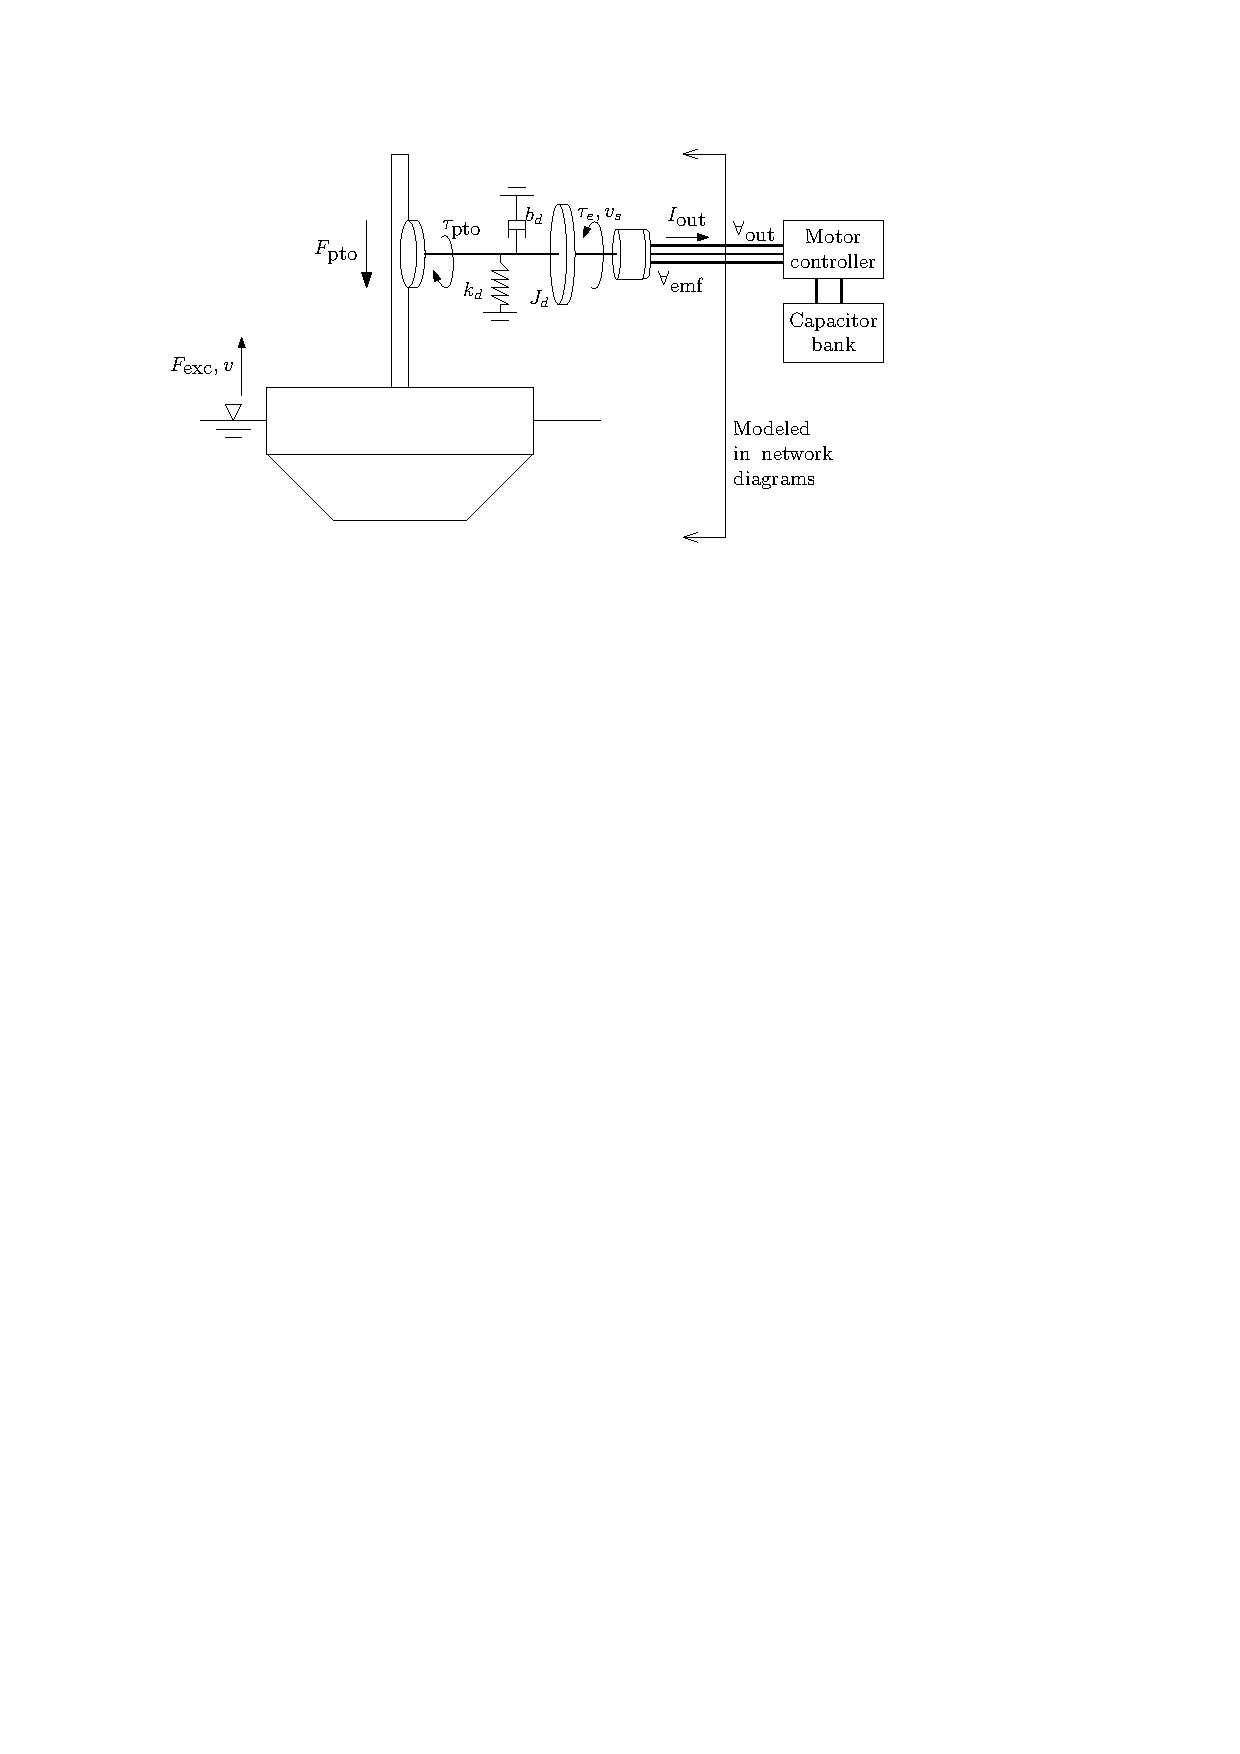
\includegraphics[width=1\columnwidth]{wec_as_multiport_phyiscal_diagram.pdf}
        \caption{WaveBot device diagram.}
        \label{fig:wec_as_multiport_phyiscal_diagram}
\end{figure}

\begin{table}[tb]
        \caption{Key physical parameters of the WaveBot.}
        \label{tab:wec_phyiscal_params}
        \centering

        \begin{tabular}{rc}
        \hline

        \hline
        \textbf{Parameter} & \textbf{Value} \\
        \hline
        Rigid body mass, $m$ [kg]                       & 875 \\
        Hydrostatic stiffness, $k_h$ [kN/m]             & 2.44 \\
        Linear friction coefficient, $b_f$ [Ns/m]       & XX \\
        Linear to rot. gear ratio, $N$ [rad/m]          & 12.4666 \\
        Shaft inertia, $J_d$ [kg\,m$^2$]                & XX \\
        Shaft friction, $b_d$ [Nm\,s/rad]               & XX \\
        Grounded shaft spring stiffness, $k_d$ [Nm/rad] & XX \\
        Torque constant, $k_\tau$ [Nm/A]                & 6.1745 \\
        Motor winding resistance, $R_w$ [$\Omega$]      & 0.5 \\
        Motor winding inductance, $L_w$ [H]             & 0 \\
        \hline

        \hline
        \end{tabular}
\end{table}

% ------------------------------------------------------------------
\subsection{Dynamic and kinematic equations}\label{sec:dynamic_and_kinematic_equations}
Vertical motion of the buoy can be expressed as a dynamic equation dependent on the PTO force ($F_{\textrm{pto}}$)\footnote{Note that we define the ``PTO'' force in the opposite direction of the excitation force and velocity as shown in \figurename~\ref{fig:wec_as_multiport_phyiscal_diagram}. This sign convention, where, as in \eqref{eq:eom_rectilinear_motion}, we have an expression of the form $Z q = F_1 - F_2$, is most common in network diagrams and control engineering and therefore used herein.}, the excitation force ($F_{\textrm{exc}}$), and the intrinsic impedance ($Z_i$) \cite{Falnes:2002aa}.

\begin{subequations}
\begin{gather}
        F_{\textrm{exc}} - F_{\textrm{pto}} = Z_i v \label{eq:eom_rectilinear_motion} \\
        Z_i(\omega) = B(\omega) + b_f + j \left( \omega \left( m + A(\omega) \right) - \frac{k_{h}}{\omega}\right)
\end{gather}
\end{subequations}

\noindent{}\noindent{}Here, $A(\omega)$ is the added mass, $B(\omega)$ is the radiation damping, $k_h$ is the hydrostatic stiffness, $b_f$ accounts for linear friction effects, and $m$ is the rigid body inertia.
The imaginary unit is $j$ and $\omega$ is the angular frequency.
A block diagram\footnote{\label{fn:block_diagrams}Note that block diagrams are related by distinct from the network diagrams used elsewhere in this paper. To emphasize this distinction, a grey fill is used for blocks in \figurename~\ref{fig:wec_as_multiport_block_diagram}.} in \figurename~\ref{fig:wec_as_multiport_block_diagram} shows the system described by \eqref{eq:eom_rectilinear_motion}.
In \figurename~\ref{fig:wec_as_multiport_block_diagram}, the PTO force is determined based on some mechanical load impedance ($Z_{\ell m}$) -- the details of this will be discussed in more detail later on.
The excitation force ($F_{\textrm{exc}}$) is determined from the excitation transfer function ($H_{\textrm{exc}}$) based on the wave elevation~($\eta$).

\begin{figure}[tb]
        \centering
        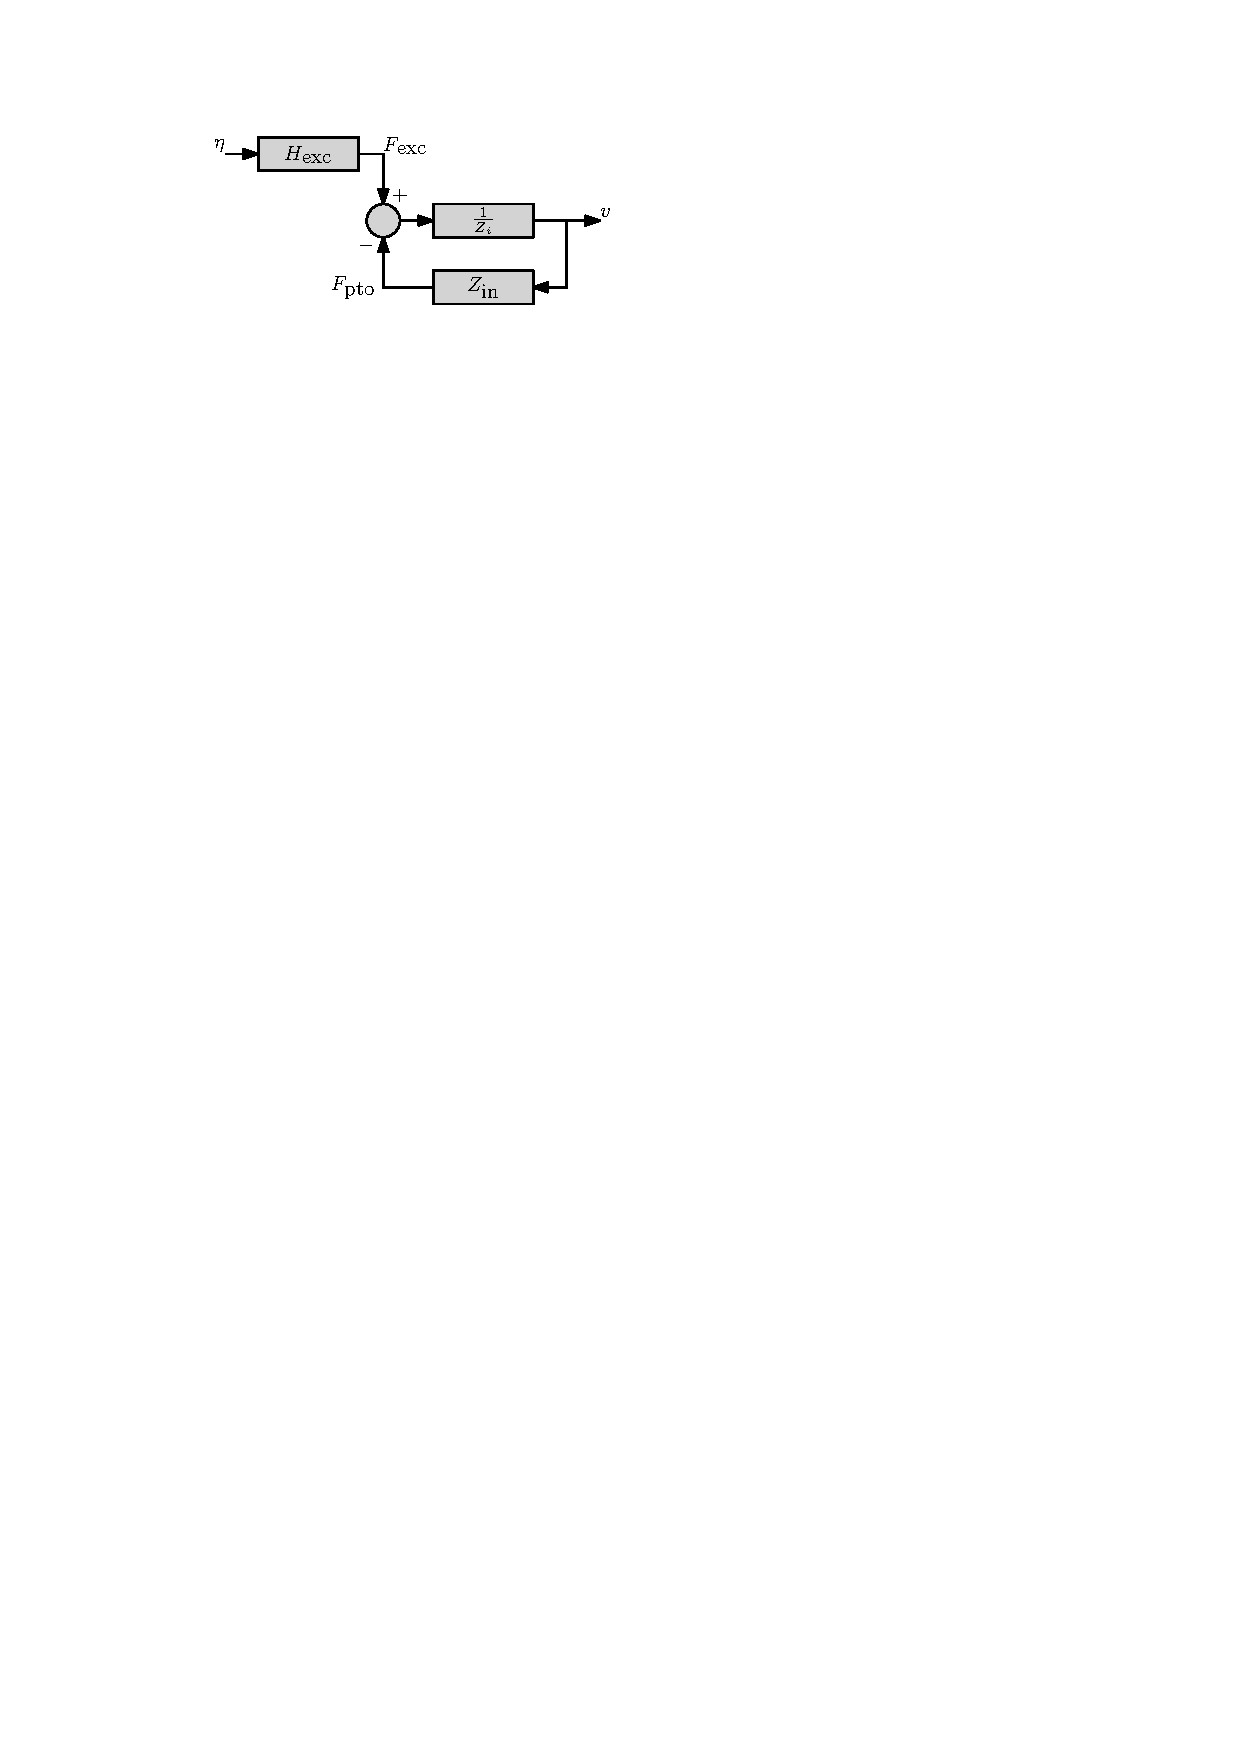
\includegraphics[width=0.8\columnwidth]{wec_as_multiport_block_diagram.pdf}
        \caption{Generic block diagram for a wave energy converter.}
        \label{fig:wec_as_multiport_block_diagram}
\end{figure}

The rectilinear vertical velocity ($v$) and force ($F_{\textrm{pto}}$) in \eqref{eq:eom_rectilinear_motion} are transformed into rotational velocity ($v_s$) and torque ($\tau_{\textrm{pto}}$) on a rotating shaft by a ``rack and pinion'' style mechanism with radius $r$.

\begin{subequations}
        \begin{gather}
                N = r \\
                v_s = N v \\
                \tau_{\textrm{pto}} = \frac{1}{N} F_{\textrm{pto}}
        \end{gather}
        \label{eq:rack_and_pinion_transmission}
\end{subequations}

\noindent{}Comparing \eqref{eq:rack_and_pinion_transmission} and \eqref{eq:transformer_eom}, we may note that the rack and pinion is an example of a transformer.

The rotating drive train shaft has a characteristic linear friction ($b_d$), inertia ($J_d$), and a may include some non-zero spring stiffness effect against ground ($k_d$).
The opposite end of the drive train shaft interfaces with an electric motor/generator that produces an electromagnetic torque ($\tau_e$).
Thus, we may describe the drive train dynamics as follows.

\begin{subequations}
        \begin{gather}
                \tau_{\textrm{pto}} - \tau_e = Z_d v_s \\
                % Z_d = i \omega J_d + b_d + \frac{k_d}{i \omega}
                Z_d = b_d + j \left( \omega J_d - \frac{k_d}{\omega} \right)
        \end{gather}
\end{subequations}

The electric motor/generator can be considered to have the composite characteristics of a pure gyrator and an impedance.
For the gyrator element, the machine has characteristic torque constant (gyration modulus) $k_\tau$ that relates back EMF voltage ($\forall_{\textrm{emf}}$) to shaft speed and electromagnetic torque to the quadrature current ($I_{\textrm{out}}$) when using a Park power invariant transformation.

\begin{subequations}
        \begin{gather}
                v_s = \frac{1}{k_\tau}\forall_{\textrm{emf}} \\
                \tau_e = k_\tau I_{\textrm{out}}
        \end{gather}
\end{subequations}

\noindent{}In addition to its gyration effect, the motor has a characteristic impedance ($Z_w$) that captures the effects of winding resistance ($R_w$) and inductance ($L_w$), and relates the output current to the back EMF voltage ($\forall_{\textrm{emf}}$) and output voltage ($\forall_{\textrm{out}}$).  \rc{-XX reference figure 6b?}

\begin{subequations}
        \begin{gather}
                \forall_{\textrm{emf}} - \forall_{\textrm{out}} = Z_w I_{\textrm{out}}\\
                Z_w = R_w + j \omega L_w \label{eq:winding_impedance}
        \end{gather}
\end{subequations}

Finally, we may define a load impedance ($Z_\ell$) that represents how current is modulated by the motor controller relative to voltage.

\begin{equation}
        Z_\ell = \frac{\forall_{\textrm{out}}}{I_{\textrm{out}}}
        \label{eq:load_impedance}
\end{equation}

\noindent{}In practice, the load impedance will be defined by a controller ($C$).
It is generally convenient to implement a feedback controller that commands motor current based on the velocity ($v$ in \figurename~\ref{fig:wec_as_multiport_phyiscal_diagram}).

\begin{subequations}
\begin{gather}
        I_{\textrm{out}} = C v \\
        Z_\ell = \frac{N}{C} k_\tau - Z_w     
\end{gather}
\end{subequations}

\noindent{}While many forms may be used for $C$, a simple proportional-integral (PI) structure, can be quite effective \cite{Coe2020a}.

\begin{equation}
        C_{PI} = v k_p + \frac{v}{j \omega} k_i \label{eq:pi_controller_structure}
\end{equation}

\noindent{}The current command in \eqref{eq:pi_controller_structure} is thus defined as the sum of products proportional to velocity ($v k_p$) and the integral of velocity ($\frac{v}{j \omega} k_i$, i.e., position).


% ------------------------------------------------------------------
\subsection{Modeling with a network diagram}\label{sec:modeling_with_a_network_diagram}

The WaveBot device shown in \figurename~\ref{fig:wec_as_multiport_phyiscal_diagram} and described in Section~\ref{sec:dynamic_and_kinematic_equations} can be represented with network diagrams as shown in \figurename~\ref{fig:wec_as_multiport_circuits}.
Various levels of abstraction and detail can be achieved in this style of diagram.
\figurename~\ref{fig:wec_as_multiport_circuits}a shows highest level of detail, whereas \figurename~\ref{fig:wec_as_multiport_circuits}b and \figurename~\ref{fig:wec_as_multiport_circuits}c increasingly combine elements to achieve a single two-port network to represent the PTO.
We will return to \figurename~\ref{fig:wec_as_multiport_circuits}d-f for later discussion.

\begin{figure}[tb]
        \centering
        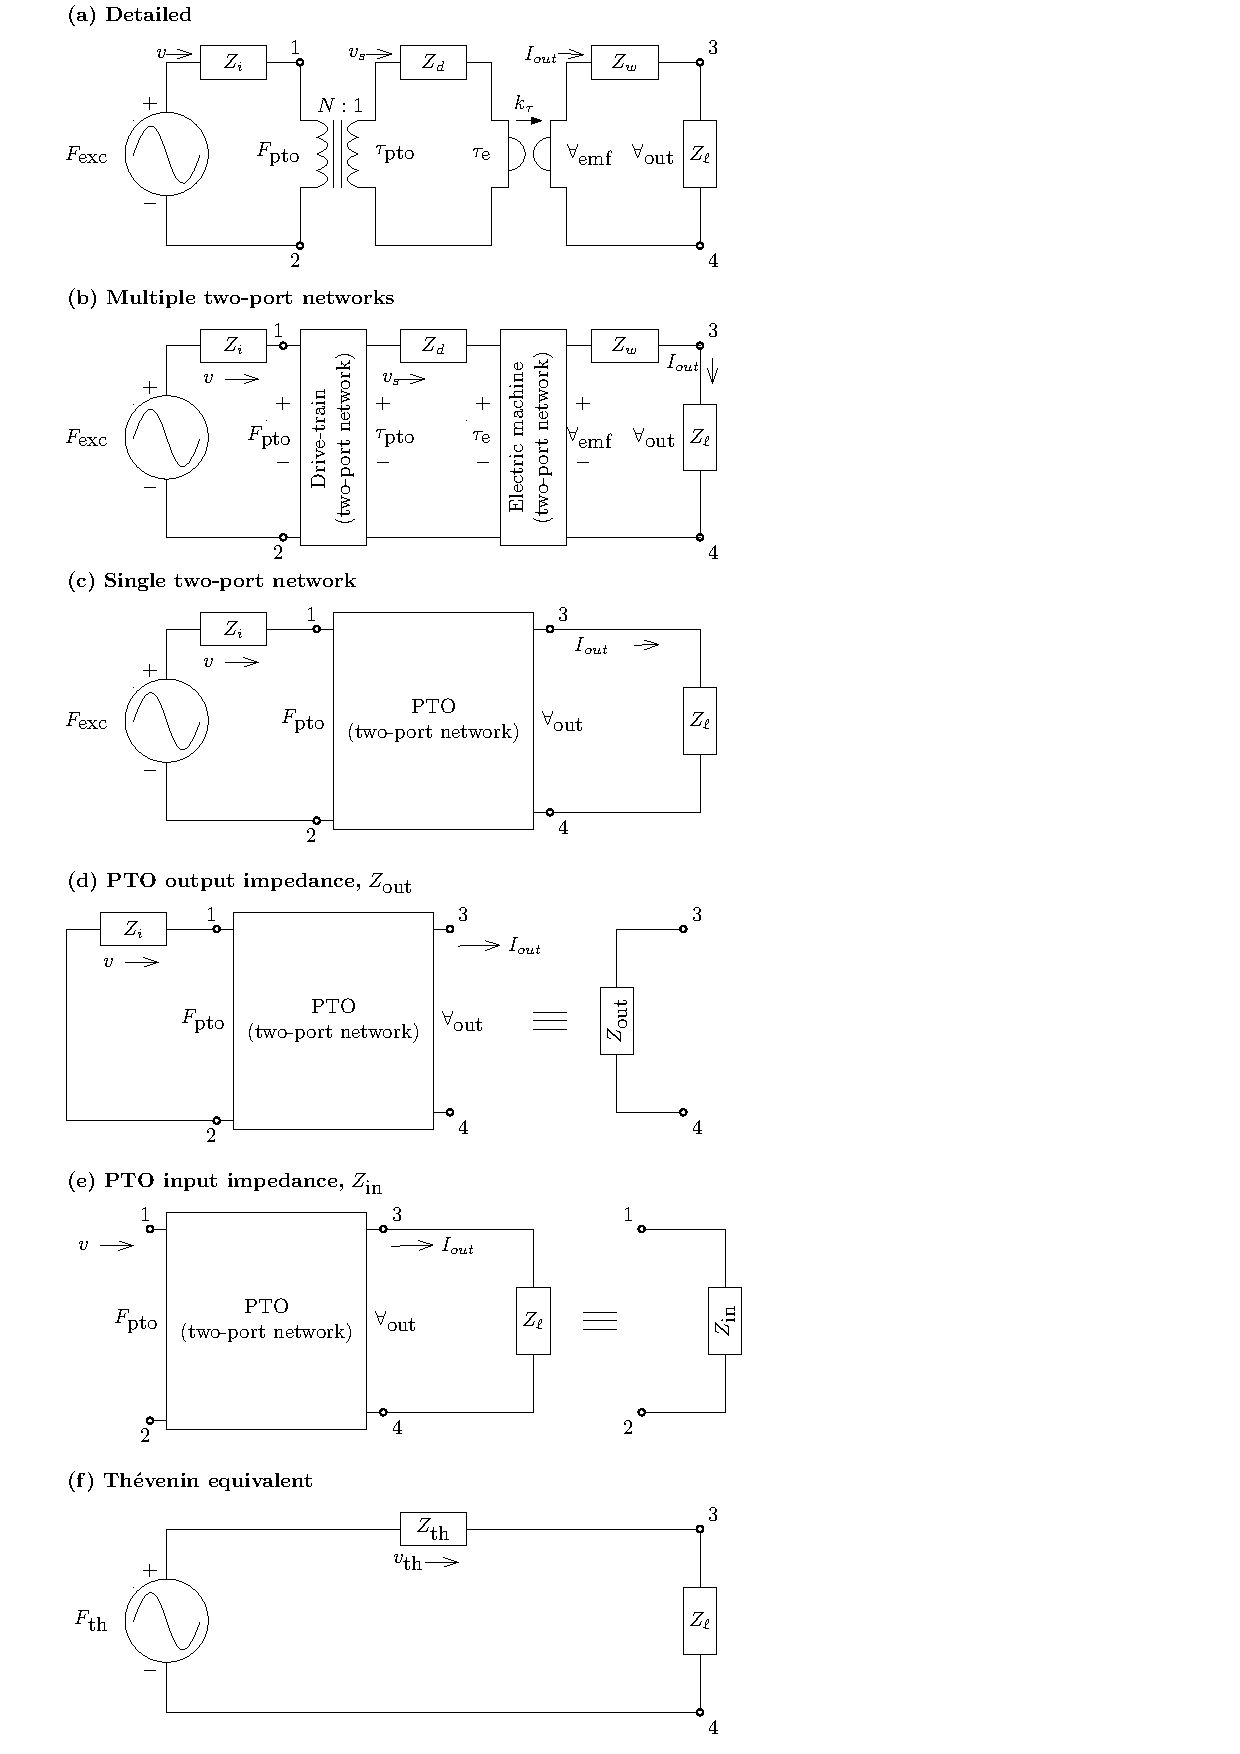
\includegraphics[width=1\columnwidth]{wec_as_multiport_circuitsv2.pdf}
        \caption{Circuit diagrams representing a wave energy converter. Points 1, 2, 3, and 4 are consistent throughout the different diagrams. \rc{XX-direction of $I_{\textrm{out}}$} \dg{XX: in b) Zd block is missing}}
        \label{fig:wec_as_multiport_circuits}
\end{figure}

\clearpage

% ------------------------------------------------------------------
\subsubsection{PTO impedance matrix}\label{sec:pto_impedance_matrix}

For the network shown in \figurename~\ref{fig:wec_as_multiport_circuits}c, we may write an impedance matrix to describe the two-port element representing the PTO.

\begin{equation}
        \label{eq:Z_mat_def}
        \begin{bmatrix} 
                F_{\textrm{pto}} \\
                \forall_{\textrm{out}} 
        \end{bmatrix} 
        = 
        \begin{bmatrix} 
                Z_{11} & Z_{12} \\ 
                Z_{21} & Z_{22} 
        \end{bmatrix} 
        \begin{bmatrix} 
                v \\
                I_{\textrm{out}} 
        \end{bmatrix} .
\end{equation}

Utilizing \eqref{eq:Z_mat_elements_def} and the equations for our system of interest presented in Section~\ref{sec:dynamic_and_kinematic_equations}, the elements of the impedance matrix in \eqref{eq:Z_mat_def} may be written out as follows.

\begin{subequations}
        \begin{align}
                &Z_{11} = \frac{e_1}{q_1} \bigg \vert_{q_2=0} 
                = \frac{F_{\textrm{pto}}}{v} \bigg \vert_{I_{\textrm{out}}=0} = Z_d \, N^2 \\[0.5em]
                %
                &Z_{12} = \frac{e_1}{q_2} \bigg \vert_{q_1=0} 
                = \frac{F_{\textrm{pto}}}{I_{\textrm{out}}} \bigg \vert_{v=0} = k_\tau \, N \\[0.5em]
                %
                &Z_{21} = \frac{e_2}{q_1} \bigg \vert_{q_2=0} 
                = \frac{\forall_{\textrm{out}}}{v} \bigg \vert_{I_{\textrm{out}}=0} = k_\tau \, N \\[0.5em]
                %
                &Z_{22} = \frac{e_2}{q_2} \bigg \vert_{q_1=0} 
                = \frac{\forall_{\textrm{out}}}{I_{\textrm{out}}} \bigg \vert_{v=0} = -Z_w 
        \end{align}
\end{subequations}

\noindent{}Taken together, this gives 

 \begin{equation}
        Z_{\textrm{pto}} 
        = 
        \begin{bmatrix} 
                Z_{11} & Z_{12} \\ 
                Z_{21} & Z_{22} 
        \end{bmatrix}
        =
        \begin{bmatrix} 
        Z_d \, N^2			& k_\tau \, N  \\
        k_\tau \, N          	& -Z_w
        \end{bmatrix}.
        \label{eq:pto_impedance}
 \end{equation}
% ------------------------------------------------------------------
\subsubsection{PTO transmission matrix}\label{sec:pto_transmission_matrix}
 The PTO impedance matrix \eqref{eq:pto_impedance} may also be arrived to by cascading the one- and two-port elements, shown in the more detailed diagram in \figurename~\ref{fig:wec_as_multiport_circuits}a and \figurename~\ref{fig:wec_as_multiport_circuits}b, by interrelating the overall transmission matrix ($ABCD$) with \eqref{eq:abcd_to_Z}.
% ------------------------------------------------------------------
\subsubsection{PTO input and output impedances}\label{sec:pto_input_and_output_impedances}

As noted in Section~\ref{sec:two_port_networks}, two-port networks may be collapsed to a one-port element if one of the ports is terminated with a load and has no independent sources.
The ``output impedance'' of the PTO ($Z_{\textrm{out}}$) is the impedance as seen by a source connected to the output port of PTO element (see \figurename~\ref{fig:wec_as_multiport_circuits}d).
As noted, we consider a scenario with no independent sources (i.e., $F_{\textrm{exc}} = 0$) and express the impedance as the ratio of effort to flow variables at the output port.

\begin{equation}
        Z_{\textrm{out}} = \frac{\forall_{\textrm{out}}}{I_{\textrm{out}}} \bigg\vert_{F_{\textrm{exc}}=0}
        \label{eq:Zout_1}
\end{equation}

\noindent{}Recalling \eqref{eq:eom_rectilinear_motion}, we may rewrite the expression for the first output in \eqref{eq:Z_mat_def} as follows.

\begin{subequations}
        \begin{align}
                F_{\textrm{pto}} = Z_{11} v + Z_{12} I_{\textrm{out}} \label{eq:Zout_Fpto_1} \\[0.5em]
                -v (Z_i + Z_{11}) = Z_{12} I_{\textrm{out}} \label{eq:Zout_Fpto_2} \\[0.5em]
                \frac{v}{I_{\textrm{out}}} = -\frac{Z_{12}}{Z_i + Z_{11}} \label{eq:Zout_Fpto_3}
        \end{align}
        \label{eq:Zout_Fpto}
\end{subequations}

\noindent{}Similarly, the expression for the second output of \eqref{eq:Z_mat_def} may be rearranged as

\begin{subequations}
        \begin{align}
                \forall_{\textrm{out}} = Z_{21} v + Z_{22} I_{\textrm{out}} \label{eq:Zout_Vout_1} \\[0.5em]
                \frac{\forall_{\textrm{out}}}{I_{\textrm{out}}} = Z_{21} \frac{v}{I_{\textrm{out}}} + Z_{22} . \label{eq:Zout_Vout_2}
        \end{align} 
        \label{eq:Zout_Vout}
\end{subequations}

\noindent{}Finally, substituting \eqref{eq:Zout_Fpto_3} into \eqref{eq:Zout_Vout_2} gives an expression for the PTO output port impedance.

\begin{equation}
        Z_{\textrm{out}} = \frac{\forall_{\textrm{out}}}{I_{\textrm{out}}} \bigg\vert_{F_{\textrm{exc}}=0} = Z_{22} - \frac{Z_{12} Z_{21}}{Z_{i} + Z_{11}}
        \label{eq:pto_output_port_impedance}
\end{equation}

The PTO input port's impedance (illustrated in \figurename~\ref{fig:wec_as_multiport_circuits}e) can be expressed as the ratio of effort ($F_{\textrm{pto}}$) and flow ($v$) on the input port.
We evaluate this scenario with input port open and with the output port fully connected such that the load impedance relates the output voltage and current.
Substituting \eqref{eq:load_impedance} into \eqref{eq:Z_mat_def} in a manner similar as was done for the output port impedance, we find

\begin{equation}
        Z_{\textrm{in}} = \frac{F_{\textrm{pto}}}{v}=  Z_{11} + \frac{Z_{12} \, Z_{21}}{Z_\ell - Z_{22}} .
        \label{eq:pto_input_port_impedance}
\end{equation}

As shown in  \cite{Bacelli:2021aa}, to maximize power transferred to the load, we can apply impedance matching at the input and output ports of the PTO.

\begin{subequations}
    \begin{align}
        Z_{\textrm{in}} = Z_i^*  \label{eq:bi_conj_matching_in} \\ 
        Z_{\textrm{out}} = Z_\ell^* \label{eq:bi_conj_matching_out}
    \end{align}
\label{eq:bi_conj_matching}
\end{subequations}

\noindent{}From \eqref{eq:bi_conj_matching}, we can explicitly see how different factors of the device design affect impedance matching and therefore power delivered to the load.
Utilizing \eqref{eq:pto_impedance}, the expressions for $Z_{\textrm{in}}$ and $Z_{\textrm{out}}$ may be expanded, giving us some insight into the design implications of the bi-conjugate impedance matching condition specified by \eqref{eq:bi_conj_matching}.

\begin{subequations}
\begin{align}
        \begin{split}
                Z_{\textrm{out}} &= Z_{22} - \frac{Z_{12} Z_{12}}{Z_{i} + Z_{11}} \\[0.5em]
                &= - Z_w - \frac{k_\tau^2 N^2}{Z_i + Z_d N^2}
        \end{split}\label{eq:expanded_zin} \\[1em]
        \begin{split}
                Z_{\textrm{in}} &= Z_{11} + \frac{Z_{12} \, Z_{21}}{Z_\ell - Z_{22}} \\[0.5em]
                &= Z_d N^2 + \frac{k_\tau^2 N^2}{Z_\ell + Z_w}
        \end{split}\label{eq:expanded_zout}
\end{align}
\end{subequations}

% ------------------------------------------------------------------
\subsubsection{Th\'{e}venin equivalent system}\label{sec:thevenin_equivalent_system}
Th\'{e}venin's theorem \cite{Thevenin:1883aa} states that any one-port network may be described by a single source ($F_{\textrm{th}}$) and impedance ($Z_{\textrm{th}}$) as shown in \figurename~\ref{fig:wec_as_multiport_circuits}e.
The Th\'{e}venin equivalent networks for WECs have been considered by a number of authors \cite{Bacelli:2021aa,Blanco:2019aa,Bubbar:2018aa,Lewis:2013aa}.
Using \eqref{eq:eom_rectilinear_motion} and the equation of the two-port network \eqref{fig:wec_as_multiport_circuits}, the following follows:
\begin{equation}
        \nonumber
        \begin{split}
                F_{\textrm{exc}} &= Z_i v + Z_{11} v + Z_{12}I_{\textrm{out}} \\
                v &= \frac{F_{\textrm{exc}} - Z_{12}I_{\textrm{out}} }{Z_i + Z_{11}} \\
                \forall_{\textrm{out}}  &= Z_{21}\left(\frac{F_{\textrm{exc}} - Z_{12}I_{\textrm{out}} }{Z_i + Z_{11}}\right) + Z_{22}I_{\textrm{out}} \\
                &= \frac{Z_{21}}{Z_i + Z_{11}} F_\textrm{exc} + \left(Z_{22} - \frac{Z_{12}Z_{21}}{Z_i + Z_{11}}\right) I_{\textrm{out}} \\
                &= F_{\textrm{th}} + Z_{\textrm{th}}I_{\textrm{out}}
        \end{split}
\end{equation}
Reviewing \figurename~\ref{fig:wec_as_multiport_circuits}e and our previous discussion about collapsing two-port elements to impedances, it becomes clear that the Th\'{e}venin equivalent impedance is equal to the PTO output impedance ($Z_{\textrm{th}} = Z_{\textrm{out}}$).
Similarly, the equivalent source can be determined by considering an effort between points 3 and 4 in \figurename~\ref{fig:wec_as_multiport_circuits} when that part of the circuit is open (i.e., no connection between points C and D) such that flow through those points is zero ($I_{\textrm{out}}=0$).
\begin{subequations}
\begin{gather}
        Z_{\textrm{th}} = Z_{\textrm{out}} = Z_{22} - \frac{Z_{21} Z_{12}}{Z_{i} + Z_{11}} \label{eq:Thevenin_impedance} \\[0.5em]
        F_{\textrm{th}} = \frac{F_{\textrm{exc}} Z_{21}}{Z_i + Z_{11}} \label{eq:Thevenin_force}
\end{gather}
\end{subequations}

We may consider the well-known impedance matching condition for the Th\'{e}venin equivalent system to design an optimal load in order to maximize the power flow from the source to the load.
\begin{subequations}
\begin{align}
        Z_\ell &= Z_{\textrm{th}}^* \\
        &= Z_{\textrm{out}}^* \label{eq:impedance_matching_thevenin_2}
\end{align} \label{eq:impedance_matching_thevenin}
\end{subequations}
\noindent{}Here, in \eqref{eq:impedance_matching_thevenin_2}, we have restated \eqref{eq:bi_conj_matching_out}.
Thus, these two modes of representing the system are indeed equivalent and give the same condition for maximum power transfer.

As illustrated in \figurename~\ref{fig:wec_as_multiport_circuits}, we may represent the WEC system in many different ways (\figurename~\ref{fig:wec_as_multiport_circuits}a, b, c, and f are all equivalent).
These different representations have different utilities.
The Th\'{e}venin equivalent system in \figurename~\ref{fig:wec_as_multiport_circuits}f is the most simplified system and gives a clear condition for control design in \eqref{eq:impedance_matching_thevenin} and a limit for maximum power delivered to the load in \eqref{eq:max_power_delivered_thevenin}.
The single two-port representation of the PTO used in \figurename~\ref{fig:wec_as_multiport_circuits}c provides an additional impedance matching condition in \eqref{eq:bi_conj_matching}, thus more clearly expressing the co-design problem.
\figurename~\ref{fig:wec_as_multiport_circuits}b provides further detail by splitting the PTO into separate drive-train and electric machine two-port elements.
While not explored in this paper, a three-part impedance matching condition could be written for the representation shown in \figurename~\ref{fig:wec_as_multiport_circuits}b.
\rc{XX-do we indeed have another matching condition if using \figurename~\ref{fig:wec_as_multiport_circuits}b? This can't logically mean that maximum power to load is $(1/2)^n$, where $n$ is the number of two-port elements}


% ------------------------------------------------------------------
\subsubsection{Power at the load}\label{sec:power_at_the_load}
Complex power delivered to the load is defined as 
\begin{equation}
\begin{aligned}
        \mathcal{S}_{\ell} 
        &= \frac{1}{2} \forall_{\textrm{out}} I_{\textrm{out}}^* \\
        &= \frac{1}{2} Z_\ell I_{\textrm{out}} I_{\textrm{out}}^* \\
        &= \frac{1}{2} Z_\ell | I_{\textrm{out}} |^2 \\
        &= \frac{1}{2} Z_\ell \left| \frac{F_{\textrm{exc}} Z_{21}}{ ( Z_{22} + Z_\ell ) (Z_i + Z_{11}) - Z_{21} Z_{12}  } \right|^2 
\end{aligned}
\end{equation}
\noindent{}We may write active, reactive, and apparent power at the load as.

\begin{subequations}
\begin{align}
&\textrm{Active: } \mathcal{P}_{\ell} = \Re \left\{ \mathcal{S}_{\ell} \right\} \\[0.5em]
&\textrm{Reactive: } \mathcal{Q}_{\ell} = \Im \left\{ \mathcal{S}_{\ell} \right\} \\[0.5em]
&\textrm{Apparent: } | \mathcal{S}_{\ell} |
\end{align}
\label{eq:load_power_types}
\end{subequations}
\noindent{}The active power is power dissipated at the load.
Returning to \figurename~\ref{fig:wec_as_multiport_phyiscal_diagram}, note that we have defined this load as the leads between the motor/generator and the motor controller.
Thus, as defined, the activate power represents power into \rc{(XX-into implies positive:good)} the motor controller.
Note that there are additional losses and dynamics in the motor controller before power is delivered to the DC bus.
However, the motor controller dynamics occur at much higher frequencies than those in the rest of the system.
For this reason, we may consider those losses separately and treat the motor controller as a static system (e.g., representing losses in the motor controller as a static function of motor torque and speed).

% \begin{equation}
% \begin{aligned}
%         G_T &= \frac{\mathcal{P}_{\ell}}{\mathcal{P}_{i}} \\
%         &= \frac{4 \left| Z_{21} \right|^2 \Re \left\{ Z_\ell \right\} \Re \left\{ Z_i \right\} }
%         {\left| (Z_{11} + Z_i)(Z_{22} + Z_\ell) - Z_{12} Z_{21} \right|^2}
% \end{aligned} \label{eq:transducer_gain}
% \end{equation}

\rc{-XX no equation $\mathcal{P}_i$ yet: probably better to present this first before obfuscating in the ratio}

When the condition \eqref{eq:bi_conj_matching_in} is satisfied, the maximum power that can be delivered to the power take-off (the input port of the two-port network) by a wave exerting an excitation force of $F_{exc}$ \cite{Falnes:2002aa} is
\begin{equation}
        \mathcal{P}_{\textrm{in,max}} = \frac{| F_{\textrm{exc}} |^2 }{ 8 \Re \left\{ Z_{\textrm{i}} \right\} }
\end{equation}
Similarly, when condition \eqref{eq:bi_conj_matching_out} is satisfied, the Th\'{e}venin equivalent system gives a clear expression for the maximum power delivered to the load.
\begin{equation}
        \mathcal{P}_{\ell\textrm{,max}} = \frac{| F_{\textrm{th}} |^2 }{ 8 \Re \left\{ Z_{\textrm{th}} \right\} }
        = \left| \frac{ Z_{21} }{ Z_i + Z_{11} } \right| ^2 \frac{ | F_{\textrm{exc}} |^2 }{ 8 \Re \left\{ Z_{\textrm{th}} \right\} } \label{eq:max_power_delivered_thevenin}
\end{equation}
If the impedances are not matched, power delivered to the power take-off $\mathcal{P}_{\textrm{in}}$ and power delievered to the load $\mathcal{P}_\ell$ are
\begin{subequations}
        \begin{align}
                \mathcal{P}_{\textrm{in}} &= \frac{1}{2} v^2 \Re \left\{ Z_{\textrm{in}} \right\}\\
                \mathcal{P}_\ell &= \frac{1}{2} I_{\textrm{out}}^2 \Re \left\{ Z_{\ell} \right\}
        \end{align}
\end{subequations}

Next, we provide three power gains (ratio of output power to input power) that are useful for system analysis. 
They are 
\begin{itemize}
        \item transducer power gain $G_T$: the ratio of power delivered to the load to the maximum power available at the source (i.e., the ``wave-to-wire efficiency'')
        \item available power gain $G_A$: the ratio of maximum power delivered to the load to the maximum power available at the source, and \ak{XX- Ideal efficiency?}
        \item operating power gain $G_O$: the ratio of power delivered to the load to the power delievered to the power take-off \ak{XX- PTO efficiency?}
\end{itemize}
\begin{subequations}
        \begin{align}
                G_T &= \frac{\mathcal{P}_\ell}{\mathcal{P}_{\textrm{in,max}}} \nonumber \\
                &= 4\left(\frac{I_{\textrm{out}}}{F_{\textrm{exc}}}\right)^2\Re \left\{ Z_i \right\}\Re \left\{ Z_{\ell} \right\}  \nonumber \\
                &= \frac{4 Z_{21}^2 \Re \left\{ Z_i \right\}\Re \left\{ Z_{\ell} \right\}}{((Z_{\ell} - Z_{22})(Z_i + Z_{11}) + Z_{12}Z_{21})^2} \label{eq:transducer_gain}
        \end{align}
        \begin{align}
                G_A &= \frac{\mathcal{P}_{\ell\textrm{,max}}}{\mathcal{P}_{\textrm{in,max}}}  \nonumber \\
                &= \left(\frac{F_{\textrm{th}}}{F_{\textrm{exc}}}\right)^2\frac{\Re \left\{ Z_i \right\}}{\Re \left\{ Z_{\textrm{th}} \right\}} \nonumber \\
                &= \left(\frac{Z_{21}}{Z_i + Z_{11}}\right)^2\frac{\Re \left\{ Z_i \right\}}{\Re \left\{ Z_{\textrm{th}} \right\}} \label{eq:available_gain}
        \end{align}
        \begin{align}
                G_O &= \frac{\mathcal{P}_\ell}{\mathcal{P}_{\textrm{in}}}  \nonumber \\
                &= \left(\frac{I_{\textrm{out}}}{v}\right)^2\frac{\Re \left\{ Z_{\ell} \right\}}{\Re \left\{ Z_{\textrm{in}} \right\}} \nonumber \\
                &=  \left(\frac{Z_{21}}{Z_{\ell} - Z_{22}}\right)^2\frac{\Re \left\{ Z_{\ell} \right\}}{\Re \left\{ Z_{\textrm{in}} \right\}} \label{eq:operating_gain}
        \end{align}
\end{subequations}


% ------------------------------------------------------------------
\section{Illustrative examples}\label{sec:illustrative_examples}
Many problems in WEC design can be considered through the concepts discussed in Section~\ref{sec:modeling_a_direct_drive_wec}.
We will consider a subset of these applications in the subsequent sections.

% ------------------------------------------------------------------
\subsection{Control design}\label{sec:control_design}
One very relevant and illustrative case is a scenario in which the machine design is considered fixed and we must maximize performance by setting the load impedance (i.e., by designing a controller).
Many papers in the area of WEC control have focused on this very problem.
In most cases, those papers consider mechanical power ($\mathcal{S}_{m}$) as the overall problem objective.

\begin{equation}
\begin{aligned}
        \mathcal{S}_{m} 
        &= \frac{1}{2} F_{\textrm{pto}} v^* \\
        &= \frac{1}{2}Z_{\ell m} v v^* \\
        &= \frac{1}{2}Z_{\ell m} | v |^2 \\
        &= \frac{1}{2} Z_{\ell m} \left| \frac{F_{\textrm{exc}}}{Z_i + Z_{\ell m}} \right|^2
\end{aligned}
\end{equation}

\noindent{}Here, we define the \emph{mechanical} load impedance as

\begin{equation}
        Z_{\ell m} = \frac{F_{\textrm{pto}}}{v} .
\end{equation}

\noindent{}Returning to \eqref{eq:pto_input_port_impedance}, we see that $Z_{\ell m}=Z_{\textrm{in}}$, thus allowing us to relate $Z_{\ell m}$ and $Z_{\ell}$.

\begin{subequations}
        \begin{gather}
                Z_{\ell m} =Z_{\textrm{in}} = Z_{11} - \frac{Z_{12} \, Z_{21}}{Z_{22} + Z_\ell} \\
                Z_\ell = \frac{Z_{12} \,Z_{21} }{Z_{11} -Z_{\ell m}}-Z_{22}
        \end{gather}
        \label{eq:Zl_Zlm}
\end{subequations}

Reflections up to the input of the PTO may be minimized by satisfy a single conjugate impedance matching condition.

\begin{equation}
        Z_i^* = Z_{\ell m}
        \label{eq:mech_power_impedance_matching}
\end{equation}

\noindent{}Not surprisingly, we see that \eqref{eq:mech_power_impedance_matching} is not dependent on the PTO impedance (i.e., this definition decouples the PTO from the control design problem).

With this in mind, it is instructive to examine the difference between controllers designed to maximize mechanical and electrical power.
\figurename~\ref{fig:wec_as_multiport_load_impedance_for_mech_power} shows the resulting load impedances for two cases:

\begin{itemize}
        \item the controller to maximize mechanical power: $Z_\ell \vert_{Z_{\ell m} = Z_i^*}$
        \item the controller to maximize electrical power: $Z_\ell = Z_{\mathrm{out}}^*$
\end{itemize}

\begin{figure}[tb]
        \centering
        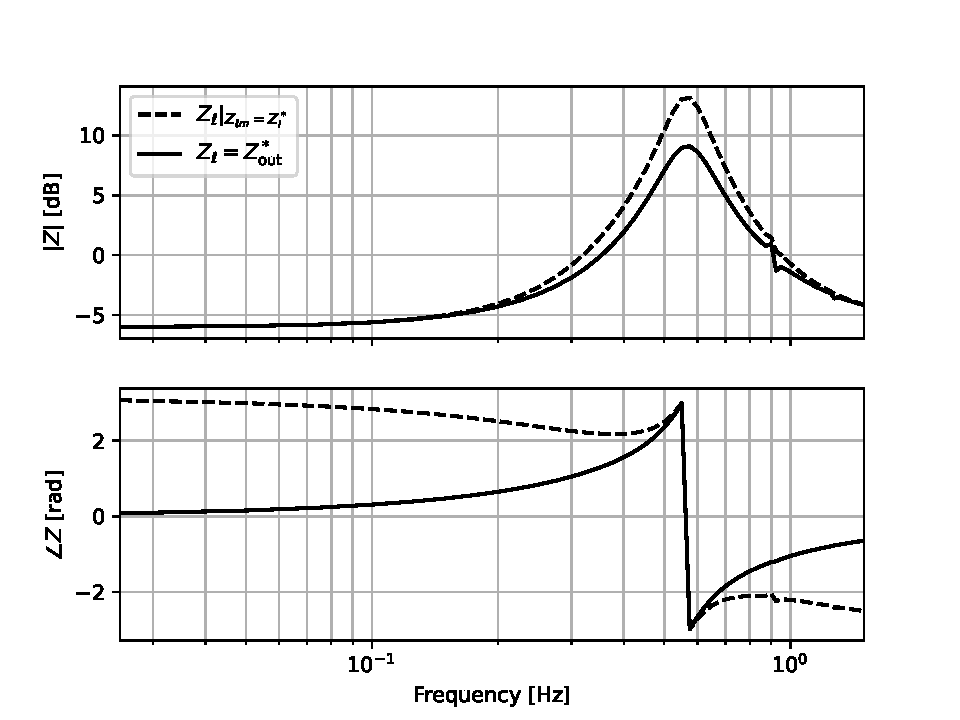
\includegraphics[width=1\columnwidth]{wec_as_multiport_load_impedance_for_mech_power_Bode.pdf}
        \caption{Load impedances (top and middle axes) created by a controller designed to maximize mechanical power ($Z_\ell \vert_{Z_{\ell m} = Z_i^*}$) and a controller designed to maximize electrical power ($Z_\ell = Z_{\mathrm{out}}^*$) along with the transducer gains (bottom axes) for each controller.}
        \label{fig:wec_as_multiport_load_impedance_for_mech_power}
\end{figure}

\noindent{}From \figurename~\ref{fig:wec_as_multiport_load_impedance_for_mech_power}, we can see that the mechanical power maximizing controller looks notably different from the controller that maximizes electrical power.
At the hydrodynamic resonance ($\sim 0.65$\,Hz), both controllers have zero phase, but the magnitudes do not match.
\rc{XX-shouldn't the electrical maximizing controller have zero phase at another frequency?}
Away from resonance, the phase of the two controllers differ dramatically.
Furthermore, the transducer gain of the two systems are dramatically different, with the gain for the mechanical power maximizing controller \emph{negative} for much of the frequency range -- this means the controller designed to \emph{maximize} mechanical power actually \emph{consumes} electrical power.

As noted in Section~\ref{sec:pto_input_and_output_impedances}, a controller is needed to realize a desired load impedance.
While higher-order controllers can \emph{approach} a perfect realization of the optimal load impedance per \eqref{eq:bi_conj_matching_out}, perfect matching at all frequencies cannot be achieved in practice\footnote{\rc{Bode-Fano limit\dots{}XX}}.
However, as noted in \cite{Coe2020a}, real ocean sea states have relatively narrow bandwidths, meaning that a given controller only need match desired load impedance matters over a narrow frequency range -- the controller can be updated to accommodate changing sea states \cite{Forbush:2022aa}.
These concepts are illustrated in \figurename~\ref{fig:gfx/wec_as_multiport_pi_controllers_real_imag}, where controllers are tuned for waves with frequencies XX, XX, and XX\,Hz.

\begin{figure}[tb]
        \centering
        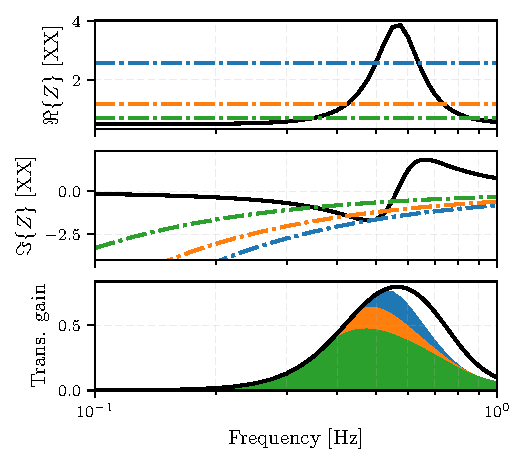
\includegraphics[width=1\columnwidth]{wec_as_multiport_pi_controllers_real_imag.pdf}
        \caption{\rc{XX-double check this}}
        \label{fig:gfx/wec_as_multiport_pi_controllers_real_imag}
\end{figure}

% ------------------------------------------------------------------
\subsection{PTO co-design}\label{sec:pto_codesign}
From \eqref{eq:bi_conj_matching}, we can see clear guidance for how the machine and controller can be designed to maximize power delivered to the load (i.e., maximize electrical power output).
Consider, for example, \figurename~\ref{fig:wec_as_multiport_in_and_out_impedances}, where we separately investigate the effects of adding a negative stiffness element\footnote{The addition of a negative stiffness has been applied by CorPower in the form a hydraulic assembly \cite{Todalshaug:2016aa} and also by Sandia Labs via a tunable magnetic spring \cite{Forbush:2024aa}.} to the drive train (\figurename~\ref{fig:wec_as_multiport_in_and_out_impedances_spring}) and adding inertia to the drive train (\figurename~\ref{fig:wec_as_multiport_in_and_out_impedances_inertia}).
The left-hand axes in each figure show $Z_{\textrm{in}}$ (colored curves) along with $Z_i^*$ (black dashed curve), which we are essentially attempting to match by altering the machine design.
The right-hand axes in each figure show $Z_{\textrm{out}}$.
In each case, we enforce \eqref{eq:bi_conj_matching_out} such the controller ($Z_\ell$) is set to maximize electrical power.

\begin{figure}
     \centering
     \begin{subfigure}[b]{1\columnwidth}
         \centering
         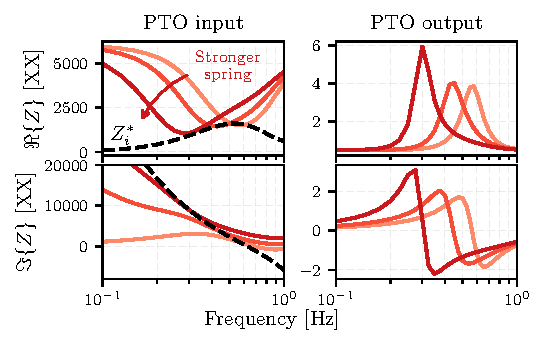
\includegraphics[width=\textwidth]{wec_as_multiport_in_and_out_impedances_spring.pdf}
         \caption{Varying levels of negative stiffness on shaft ($K_d$)}
         \label{fig:wec_as_multiport_in_and_out_impedances_spring}
     \end{subfigure}
     \\
     \begin{subfigure}[b]{1\columnwidth}
         \centering
         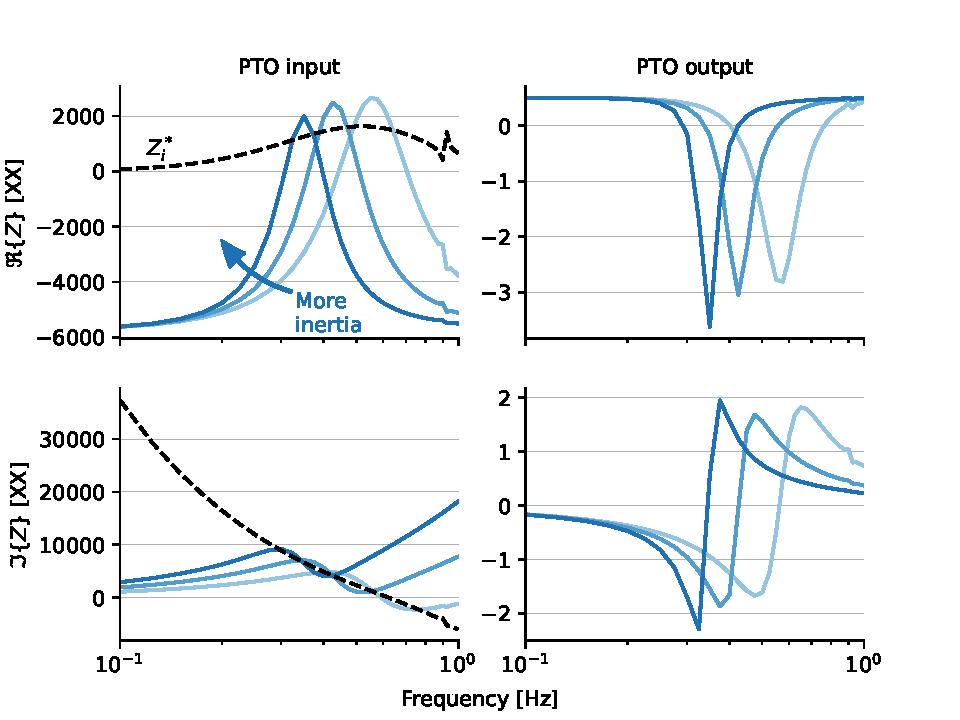
\includegraphics[width=\textwidth]{wec_as_multiport_in_and_out_impedances_inertia.pdf}
         \caption{Varying levels of shaft inertia ($I_d$)}
         \label{fig:wec_as_multiport_in_and_out_impedances_inertia}
     \end{subfigure}
     \caption{Input port (left) and output port (right) impedances. Upper axes show real part ($\Re \{ Z \}$), lower axes show imaginary part ($\Im \{ Z \}$). Impedance matching condition on the input port per \eqref{eq:bi_conj_matching_in} illustrated by black dashed curve.}
     \label{fig:wec_as_multiport_in_and_out_impedances}
\end{figure}


Both of the considered design alterations (negative stiffness and increased shaft inertia) have the effect of improving impedance matching on the input port at lower frequencies.
Recall also that the power transported by an ocean wave is inversely proportional to the wave frequency ($J \propto f^{-1}$) such that this improved impedance matching at lower frequencies may be particularly advantageous.
It should be noted that the range of values for $K_d$ and $I_d$ shown in \figurename~\ref{fig:wec_as_multiport_in_and_out_impedances} is somewhat arbitrary and intended only to illustrate trends -- one cannot directly compare the effects of doubling the shaft inertia with doubling the negative spring stiffness in terms of an engineering decision.
With this in mind, we can see that, for this specific example, adding shaft inertia (\figurename~\ref{fig:wec_as_multiport_in_and_out_impedances_inertia}) appears to adversely affect the shape of the input impedance (both in terms of the real and imaginary parts) by narrowing the bandwidth over which a good matching with the intrinsic impedance is achieved, whereas adding a negative spring (\figurename~\ref{fig:wec_as_multiport_in_and_out_impedances_inertia}) appears to have the opposite affect, generally increasing the bandwidth over which good matching with the intrinsic impedance occurs.


While based on \eqref{eq:drive_train_impedance} we might expect changes to $K_d$ and $I_d$ to only affect the imaginary part of the impedances, we may see by expanding \eqref{eq:pto_output_port_impedance} and \eqref{eq:pto_input_port_impedance} that these terms do indeed effect the real part of the impedances as shown in \figurename~\ref{fig:wec_as_multiport_in_and_out_impedances}.
\rc{XX-reference expanded versions of these equations}

\noindent{}Note that in \eqref{eq:expanded_zout}, we have left $Z_{\textrm{out}}^*$ unexpanded, but one can see rather clearly see by referencing \eqref{eq:expanded_zin} how the drive train stiffness ($K_d$) and inertia ($I_d$) enter in.

\rc{
\begin{itemize}
        \item XX-as $| \Im \{ Z_\ell \} |$ increases within the frequency range of interest\dots{}
        \begin{itemize}
                \item More reactive power
        \end{itemize}
        \item XX-as $| \Re \{ Z_\ell \} |$ increases within the frequency range of interest\dots{}
        \begin{itemize}
                \item Higher feedback gains, more challenges with stability/sensitivity
        \end{itemize}
\end{itemize}}

The resulting performance of these different designs can be characterized using the transducer gain defined in \eqref{eq:transducer_gain}, as shown in \figurename~\ref{fig:wec_as_multiport_spring_inertia_transducer_gains}.
As noted from \figurename~\ref{fig:wec_as_multiport_in_and_out_impedances}, the negative spring creates a broader impedance matching, and thus we observe that the ``wave-to-wire'' efficiency for the spring designs than the shaft inertia designs.
Of course that we do not need to apply these design strategies exclusively, and that in practice we would consider altering the shaft inertia and negative spring effect.
Different WEC archetypes will have different design parameters; for example, an oscillating water column design could consider the shaft inertia, air chamber volume (related to stiffness), and many other factors.

\begin{figure}[tb]
        \centering
        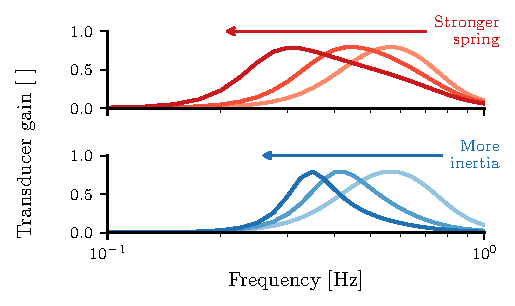
\includegraphics[width=1\columnwidth]{wec_as_multiport_spring_inertia_transducer_gains.pdf}
        \caption{\rc{XX-improve colors} \rc{XX-add legend or arrows?}}
        \label{fig:wec_as_multiport_spring_inertia_transducer_gains}
\end{figure}

% ------------------------------------------------------------------
\subsection{Steady input}\label{sec:steady_input}
Much of the theory presented here could be interpreted to indicate that WECs are a special case amongst energy conversion systems when compared with, e.g., wind turbines, which utilize a mostly steady power input.
However, it is actually the opposite: the bi-conjugate impedance matching condition given by \eqref{eq:bi_conj_matching} is general and the steady input energy conversion systems are a special case of that general theory.

Assuming a similar PTO architecture, the expressions XX remain the same.
The fundamental difference is that the excitation is steady ($\Im \{ Fe \} = 0$) and has no frequency dependence.

\rc{
XX-show that, for a wind turbine, \eqref{eq:bi_conj_matching} reduces to minimizing losses -- actually not sure if this follows from \eqref{eq:bi_conj_matching} or not? -- and setting $Z_\ell$ to some real value.
XX-How does reducing the real part of the impedance factor in?}

\begin{equation}
        \mathcal{P}_{in} = \frac{ | F_{\textrm{exc}} |^2 }{8 \Re \{ Z_i \}}
\end{equation}

\rc{XX-Perhaps you must also consider how changes in $Z_i$ affect $H$ (and therefore $F_{\textrm{exc}}$)?
XX-The Haskind relations connect the excitation transfer function and radiation damping ($\Re \{ Z_i \}$) \cite[pg. 304]{Newman:1978aa}.
For example, for a symmetric 2D body,}

\begin{equation}
        B_{ii}(\omega) = \frac{| H_{ii} |^2}{2 \rho g v_g} .
\end{equation}

\rc{
\noindent{}Alternatively, Falnes presents \cite[pg. 149]{Falnes:2002aa} the following for an axisymmetric body in heave.}

\begin{equation}
        B_{33}(\omega) = \frac{k}{8J} | F_{e,3} |^2
\end{equation}

\rc{
\noindent{}Therefore, increases in the radiation damping result in quadratic increases in the excitation transfer function.
XX-cross flow turbines and flapping devices\dots{}
\begin{itemize}
        \item Input power is steady? - or is it oscillatory once you get moving?
        \item Doesn't this mean that by oscillating you are creating a mismatch?
        \item Gust control for wind turbines - they inject power to speed up, if analyzed in the frequency domain, this is impedance conjugate matching controller
\end{itemize}}


% \cleardoublepage
% % ------------------------------------------------------------------
% \section{xx}


% \begin{subequations}
%         \begin{align}
%         Z_d \, v_s = \tau_e + \tau_{\textrm{pto}} \\
%         F_{\textrm{pto}} = \tau_{\textrm{pto}} \, N \\
%         v = \frac{1}{N} v_s 
%         \end{align}
%         \label{eq:drive_train_dynamics}
% \end{subequations}

% \noindent{}Here, $v_s$ is the shaft speed, which is related to the hull velocity $v$ by the gear ratio $N$.
% Similarly, the gear ratio relates the force on the hull from the PTO ($F_{\textrm{pto}}$) to the output torque from the PTO shaft ($\tau_{\textrm{pto}}$).
% This output torque $\tau_{\textrm{pto}}$ is due to the electrical torque produced by the motor/generator ($\tau_e$) and a passive effect described by the drive train impedance ($Z_d$).

% \begin{equation}
%         Z_d = i \omega I_d  + B_d  + \frac{K_d}{i \omega}
%         \label{eq:drive_train_impedance}
% \end{equation}


% To relate the electrical torque and shaft speed to the motor current and voltage, we apply the power-invariant Park transform \cite{Park:1929aa} \rc{XX-explain why}.

% \begin{subequations}
%     \begin{align}
%         &\tau_e = -  \sqrt{\frac{3}{2}} k_\tau  I_{\textrm{out}} ,                               \label{eq:gen_iq_model} \\[0.5em]
%         &\forall_{\textrm{out}} = \sqrt{\frac{3}{2}} k_\tau v_s +  Z_w I_{\textrm{out}} .        \label{eq:gen_vq_model}
%     \end{align}
% \label{eq:park_transform}
% \end{subequations}

% \noindent{}Here, the variable $k_\tau$ is the motor torque coefficient.
% The motor winding impedance in \eqref{eq:gen_vq_model} is defined by the winding resistance ($R_w$) and inductance ($L_w$).

% \begin{equation}
%         Z_w = R_w + j \omega L_w
%         \label{eq:winding_impedance}
% \end{equation}


% We may now conceptualize the ``wave-to-wire'' WEC system as the network shown in \figurename~\ref{fig:wec_as_multiport_circuits}.
% On the far left hand side of \figurename~\ref{fig:wec_as_multiport_circuits}, we have the oscillating effort $F_{\textrm{exc}}$.


% Utilizing these relationships, the elements of the impedance matrix in \eqref{eq:Z_mat_def} written out as \rc{XX-explain definitions}




% \begin{subequations}
%         \begin{align}
%                 &Z_{11} = \frac{e_1}{q_1} \bigg \vert_{q_2=0} 
%                 = \frac{F_{\textrm{pto}}}{v} \bigg \vert_{I_{\textrm{out}}=0} = Z_d \, N^2 \\[0.5em]
%                 %
%                 &Z_{12} = \frac{e_1}{q_2} \bigg \vert_{q_1=0} 
%                 = \frac{F_{\textrm{pto}}}{I_{\textrm{out}}} \bigg \vert_{v=0} = -\sqrt{\frac{3}{2}}k_\tau \, N \\[0.5em]
%                 %
%                 &Z_{21} = \frac{e_2}{q_1} \bigg \vert_{q_2=0} 
%                 = \frac{\forall_{\textrm{out}}}{v} \bigg \vert_{I_{\textrm{out}}=0} = -\sqrt{\frac{3}{2}}k_\tau \, N \\[0.5em]
%                 %
%                 &Z_{22} = \frac{e_2}{q_2} \bigg \vert_{q_1=0} 
%                 = \frac{\forall_{\textrm{out}}}{I_{\textrm{out}}} \bigg \vert_{v=0} = Z_w .
%         \end{align}
% \end{subequations}

% \noindent{}Taken together, this gives 

%  \begin{equation}
%         Z_{\textrm{pto}} 
%         = 
%         \begin{bmatrix} 
%                 Z_{11} & Z_{12} \\ 
%                 Z_{21} & Z_{22} 
%         \end{bmatrix}
%         =
%         \begin{bmatrix} 
%         Z_d \, N^2                              & -\sqrt{\frac{3}{2}}k_\tau \, N  \\
%         -\sqrt{\frac{3}{2}}k_\tau \, N          & Z_w
%         \end{bmatrix}.
%         \label{eq:pto_impedance}
%  \end{equation}

%  \noindent{}Note that \eqref{eq:pto_impedance} is in ``impedance form'' -- other forms of multi-port network representations can useful depending on the application.
%  For example, the ``$ABCD$ form'' allows for the straightforward cascading two-port networks (see, e.g., \cite{Frickey:1994aa}).

% % \begin{align}
% %         \tau_e &= - \sqrt{\frac{3}{2}} k_\tau \, i                 \label{eq:gen_iq_model}\\
% %         v &= \sqrt{\frac{3}{2}} k_\tau \Omega + Z_w i              \label{eq:gen_vq_model}
% % \end{align}




% % i \omega I_d  + B_d  + \frac{K_d}{i \omega}
% % R_w + j \omega L_w

%Initial efforts at WEC control optimization borrowed from wind and tidal energy control, which as shown, offers imperfect power capture.
The obvious contrast is that wind and tidal energy flows contain the majority of their energy in slowly-varying ``mean'' flows: though the frequency-domain characteristics of turbulence may be characteristically similar to wave spectra, they contain significantly less energy in viable wind/tidal/current energy sites, the fitness of which are determined primarily from the magnitude of the slowly-varying (i.e., hours to days) velocity components.
Consider this tidal cycle taken over 24 hours from a deployed acoustic doppler velocimeter in Admiralty Inlet, WA (\cite{NREL2015}, \figurename~\ref{fig: TidalVelocity}).

\begin{figure}
	\centering 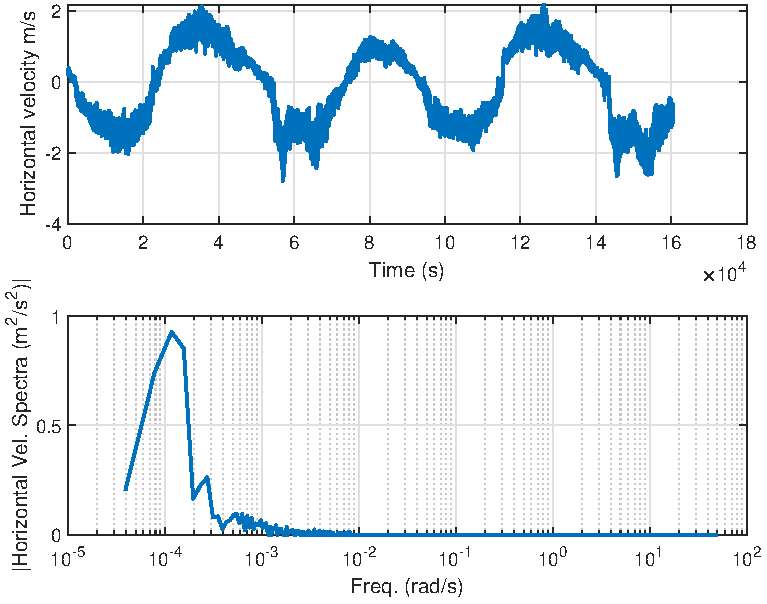
\includegraphics[width=\columnwidth]{TidalVelocity.pdf}
	\caption{Acoustic doppler velocimeter data from an approximately 45 hour deployment in Admiralty Inlet, WA.
	Sampled at 16 Hz.}
	\label{fig: TidalVelocity}
\end{figure}

However, a wind/tidal turbine can be similarly decomposed into a transfer function representation as per \figurename~\ref{fig:wec_as_multiport_block_diagram}, where the wind/water speed $U$ exerts a torque on the rotor $\tau_h$ which is summed with a controller torque $\tau_{pto}$, and the intrinsic impedance of the rotor and drivetrain are

\begin{subequations}
		
	\begin{gather}
		Z_{turb,i}(\omega)=b_f + j\omega J_{turb} \\
		Z_{turb,d}(\omega)=b_d + j\omega J_d
	\end{gather}
\end{subequations}

\noindent{respectively, and the motor/generator impedance is described as \ref{eq:winding_impedance}.
Note that the excitation force exerted from fluid velocity $U$, is a non-linear function, but may be approximated as linear over small perturbations.
While representing a non-linear rotor system as a first-order transfer function is an abstraction, it is a useful model when one considers that a family of first-order models linearized about different rotor operating points could reasonably approximate overall system dynamics, and each of those first-order models will be characteristically similar to those presented here: these conclusions are at least qualitatively valid over stable rotor operating states.
	
Considering the rotor itself, a gearbox, internal drivetrain components, and a motor/generator, the wind/tidal turbine system can also be described as the two-port networks in \figurename~\ref{fig:wec_as_multiport_circuits}.
Following the derivations in the the preceeding sections we arrive again at the following bi-conjugate impedance matching conditions expressed in Equations \eqref{eq:expanded_zin} and \eqref{eq:expanded_zout}}.
Considering $Z_L$, we again aim to maximize electrical power delivered to the load (i.e., ``Region 2 control'' \cite{Handbook2011}), and to preserve generality we consider feedback controllers of the form above (Eq.
\ref{eq:pi_controller_structure}), in which $\tau_{pto}$ is determined from a measurement rotor angular velocity $\omega$.
These conditions are plotted using parameters summarized in Table \ref{tab:tidal phyiscal_params} in \figurename~\ref{fig: RotorZinZout}.


\begin{table}[tb]
	\caption{Parameters of the hypothetical tidal power system.}
	\label{tab:tidal phyiscal_params}
	\centering
	
	\begin{tabular}{rc}
		\hline
		
		\hline
		\textbf{Parameter} & \textbf{Value} \\
		\hline
		Rotor friction $b_f$ [Nm\_s/rad] & 1 \\
		Rotor inertia $J_{turb}$ [kg-m$^2$] & 10 \\
		Gear ratio, $N$ [rad/rad] & 12.4666 \\
		Shaft inertia, $J_d$ [kg\,m$^2$]                & 1 \\
		Shaft friction, $b_d$ [Nm\,s/rad]               & 0.1 \\
		Torque constant, $k_\tau$ [Nm/A]                & 6.1745 \\
		Motor winding resistance, $R_w$ [$\Omega$]      & 0.1 \\
		Motor winding inductance, $L_w$ [H]             & 0.1 \\
		\hline
		
		\hline
	\end{tabular}
\end{table}

\begin{figure}
	\centering 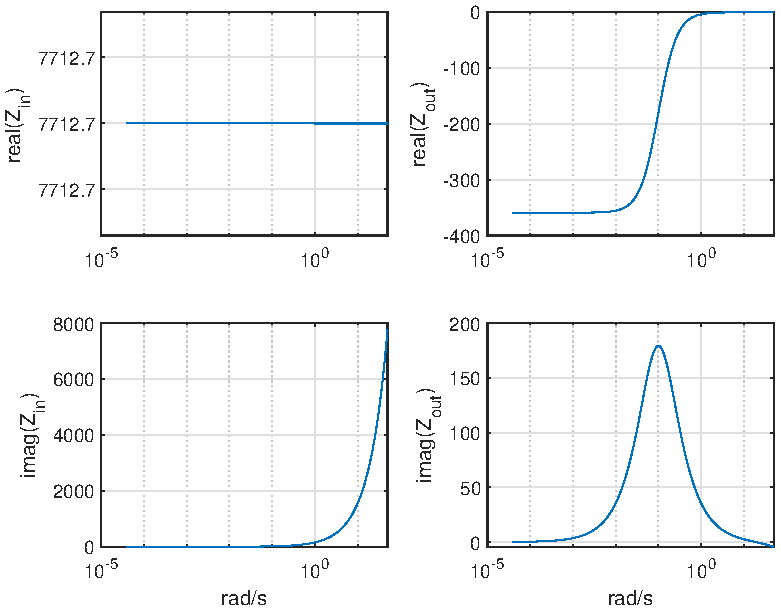
\includegraphics[width=\columnwidth]{RotorZinZout.pdf}
	\caption{Real (top) and imaginary (bottom) parts of the input (left) and output (right) impedance.}
	\label{fig: RotorZinZout}
\end{figure}

The key characteristic difference in the appearance of the input and output impedances is the absence of a stiffness-type term in the intrinsic and drivetrain impedances, implying that these are now first-order systems.
Note that over the energy-containing frequencies of the flow, that the imaginary part of both $Z_{in}$ and $Z_{out}$ are zero, implying that a damping-type controller will be optimal over these frequencies \eqref{eq:bi_conj_matching_out} and that the co-design problem is the proper selection of $N$ and $K_T$ and the minimization of friction losses $B$ and $B_d$ \eqref{eq:bi_conj_matching_in}, \eqref{eq:bi_conj_matching_out}.
Though co-design for wind/tidal rotors is not typically formalized in this way, note that the common wind turbine control algorithm $\tau_{pto} = K\omega^2$, where $K$ is a constant determined from the aerodynamic parameters of the rotor, is effectively a non-linear damper for which there is no reactive control term.
Further, towards higher frequencies where the imaginary part of $Z_{out}$ increases, the optimal controller will need positive phase (e.g., a lead compensator) to capture any excitation present at these frequencies: in fact, state-of-the-art wind turbine controllers use an ``upstream'' measurement or model of accelerations in free-stream velocity and adjust rotor state ahead of time to maximize power capture of the stochastically varying free-stream turbulence \cite{Schlipf2013b}.
Under these conditions, bi-conjugate impedance matching conditions become increasingly relevant, but are still not commensurately critical as their application to wave energy where the vast majority of the available energy is not contained in a ``steady'' mean flow (or one that varies at frequencies much lower than the device dynamics).

Considering the selection of $N$ and $K_T$ values, the appropriate gear ratio is more probably driven by the combined consideration of 1) an efficient generator operating speed and torque and 2) the designed tip-speed ratio of the rotor (and its implied $\omega$ in a given $U$).
If the non-linear fluid excitation of the rotor is taken as guidance in these design decisions, which over excited frequencies affects the real part most significantly, then bi-conjugate impedance matching conditions simplify further to the minimization of friction losses $B$ and $B_d$.

In this way, we see that the underlying theory is, with some linearizing approximations, valid for the power capture of wind/tidal turbines as well, but bi-conjugate impedance matching conditions are simpler to achieve over the energetic frequency bands and historically did not need to be considered explicitly for efficient energy capture because the frequency ranges over which device and PTO dynamics become important tend to be significantly higher.
Secondly, the nonlinearities of the aerodynamic system lead to more convenient power-maximizing control formulations in the time-domain.


% ------------------------------------------------------------------
\section{Discussion and conclusions}
The interrelated nature of the WEC design process becomes quite clear when viewed as an impedance matching problem.
In practice, the bi-conjugate impedance matching requirement expressed by \eqref{eq:bi_conj_matching} cannot be perfectly satisfied at all frequencies and the cost of improving the matching condition must be balanced with the resulting benefits.
Furthermore, this formulation does not capture constraints (e.g., maximum torque from a generator or maximum travel of a linear piston) and nonlinear dynamics, which eventually must be considered.
Given these practical considerations, numerical optimization becomes a useful tool becomes useful in practice.
Nonetheless, the linear modeling approach presented here provides a critical starting point and foundation to build from.

% ------------------------------------------------------------------
\section{Acknowledgements}
The authors would like to acknowledge funding support from the US Department of Energy's Water Power Technologies Office.
Sandia National Laboratories is a multi-mission laboratory managed and operated by National Technology and Engineering Solutions of Sandia, LLC., a wholly owned subsidiary of Honeywell International, Inc., for the U.S. Department of Energy's National Nuclear Security Administration under contract DE-NA0003525.
This paper describes objective technical results and analysis.
Any subjective views or opinions that might be expressed in the paper do not necessarily represent the views of the U.S. Department of Energy or the United States Government.

% ------------------------------------------------------------------
\bibliographystyle{IEEEtran}
\bibliography{wec_as_multiport.bib}


\begin{IEEEbiography}[{
\includegraphics[width=1in,height=1.25in,clip,keepaspectratio]{author_photos/RyanCoe.jpg}}]{Ryan G. Coe}
received a B.S. degree in Ocean Engineering (2009) and a Ph.D. in Aerospace Engineering (2013), both from Virginia Tech.
He subsequently joined Sandia National Laboratories' Water Power Technologies group in 2013.
Ryan's research focuses primarily on wave energy converter (WEC) modeling, control, testing, and design.
Ryan is an Associate Editor for the \emph{Journal of Waterway, Port, Coastal, and Ocean Engineering} and the \emph{Journal of Ocean Engineering and Marine Energy} and an Editorial Board member for \emph{Energies}; he also serves as Convenor for the International Electrotechnical Commission (IEC) on the subject of ''Design requirements for marine energy systems.''
\end{IEEEbiography}

\begin{IEEEbiography}[{
\includegraphics[width=1in,height=1.25in,clip,keepaspectratio]{author_photos/GiorgioBacelli.jpg}}]{Giorgio Bacelli} received his master's degree from Università Politecnica delle Marche and his PhD from the National University of Ireland, Maynooth. 
He is a senior research engineer in the Water Power Technologies Department at Sandia National Laboratories, where the focus of his research is on the dynamics and control of wave energy converters, power take off design and experimental testing.
He serves as a Subject Matter Expert (SME) for International Electrotechnical Commission (IEC) on the subject of ``Guidelines for the early stage development of wave energy converters.''
\end{IEEEbiography}

\begin{IEEEbiography}[{
\includegraphics[width=1in,height=1.25in,clip,keepaspectratio]{author_photos/DominicForbush_cropped.jpg}}]{Dominic Forbush}
is a senior research and development engineer in the Water Power Technologies Program at Sandia National Laboratories.
Dominic's research focuses on the control, modeling, and the development of innovative solutions for wave energy converters (WECs).
Particularly, Dominic is involved in developing and supporting open-source WEC modeling tools, wave tank testing of WEC devices and control approaches, and the application of structured innovation techniques to the wave energy space.
Dominic has a bachelor's, master's, and doctorate all in mechanical engineering from the University of Washington, where his graduate work focused on the control of cross-flow hydrokinetic turbines.
\end{IEEEbiography}

\begin{IEEEbiography}[{
\includegraphics[width=1in,height=1.25in,clip,keepaspectratio]{author_photos/DanielGaebele.jpg}}]{Daniel T. Gaebele}
received his B.S., and M.S. in Engineering Cybernetics (2015, and 2018) from the University of Stuttgart, Germany, and a Ph.D. in Electrical and Computer Engineering (2021) from Oregon State University.
He joined Sandia National Laboratories' Water Power Technologies Department as a Postdoctoral Appointee in 2021.
His researches focuses on wave energy converter (WEC) co-optimization and the sociotechnical assessments of WECs for Blue Economy applications.
\end{IEEEbiography}

\begin{IEEEbiography}[{
\includegraphics[width=1in,height=1.25in,clip,keepaspectratio]{author_photos/AliciaKeow.jpg}}]{Alicia Keow}
is a postdoctoral appointee in the Water Power Technologies Program at Sandia National Laboratories.
Her research focuses on the use of control co-design methodologies to develop next generation Marine Hydrokinetic (MHK) systems.
Alicia received her bachelor's degree in electrical engineering from Wichita State University in 2016, and her PhD in mechanical engineering from the University of Houston in 2021.
\end{IEEEbiography}

\end{document}


